%!TEX root = IntroArithGrps.tex


\mychapter{\texorpdfstring{Examples of\\Arithmetic Groups}%
	{Examples of Arithmetic Groups}}
\label{EgArithGrpsChap}

\prereqs{definition of arithmetic subgroup (\cref{ArithLattDefnSect}), Godement Criterion (\cref{GodementCriterion}), and restriction of scalars (\cref{RestrictScalarsSect}).}

\section{Arithmetic subgroups of \texorpdfstring{$\SL(2,\real)$}{SL(2,R)} via orthogonal groups} 
\label{ArithLattSL2}

$\SL(2,\integer)$ is the obvious example of an arithmetic
subgroup of $\SL(2,\real)$. Later in this section, we will show that (up to
commensurability and conjugates) it is the only one that is
not cocompact \csee{NoncocpctSL2R=SL2Z}. In contrast, there are infinitely many
cocompact, arithmetic subgroups. They can be constructed by
several different methods. Perhaps the easiest way is to
note that $\SL(2,\real)$ is isogenous to the special orthogonal group $\SO(2,1)$. 

\begin{notation} \label{SO3wayNotation}
In this chapter (and others), we will see many different special orthogonal groups over a field~$F$.
They can be specified in (at least) three different, but equivalent ways:
	\begin{enumerate}
	
	\item (\term{Gram matrix}) For a symmetric, invertible matrix $A \in \Mat_{\ell \times \ell}(F)$, we define
	$$ \SO(A;F) = \{\, g \in \SL(n,F) \mid g^\transpose A g = A \,\} .$$
	This is the approach taken to the definition of $\SO(m,n)$ in \cref{classical-fulllinear}.

	\item (\term[bilinear form]{Bilinear form}) A symmetric, bilinear form~$B$ on~$F^\ell$ is \defit[nondegenerate!bilinear form]{nondegenerate} if, for all nonzero $v \in F^\ell$, there exists $w \in F^\ell$, such that $B(v,w) \neq 0$. We define
	$$ \SO(B;F) = \{\, g \in \SL(\ell,F) \mid B(gv,gw) = B(v,w), \ \forall v,w \in F^\ell \,\} .$$

	\item ({Quadratic form}) A \defit{quadratic form} on~$F^\ell$ is a homogeneous polynomial $Q(x_1,\ldots,x_\ell)$ of degree~$2$.  It is \defit[nondegenerate!quadratic form]{nondegenerate} if the corresponding bilinear form $B_Q$ is nondegenerate, where
	$$ B_Q(v,w) = {\textstyle\frac{1}{4}} \bigl( Q(v + w) - Q(v - w) \bigr) .$$
	We define
	 $$ \SO(Q;F) = \{\, g \in \SL(\ell,F) \mid Q(gv) = Q(v), \ \forall v \in F^\ell \,\} .$$

	\end{enumerate}
The three approaches give rise to exactly the same groups \csee{SO3ways}, and it is straightforward to translate between them, so we will use whichever notation is most convenient in a particular context.
\end{notation}	

\begin{egs} \label{ArithSO21Eg} \ 
\noprelistbreak
 \begin{enumerate}
 \item \label{ArithSO21Eg-Q}
 Fix positive integers $a$ and~$b$, and let 
 $$G = \SO(a x^2 + b y^2 - z^2; \real) \iso
\SO(2,1) .$$
 If $(0,0,0)$ is the only integer solution of the
Diophantine equation $a x^2 + b y^2 = z^2$, then
$G_{\integer}$ is a cocompact, arithmetic subgroup of~$G$
\csee{anis->cocpct}. See \cref{px2+py2<>z2} for some
examples of $a$ and~$b$ satisfying the hypotheses.
 \item Restriction of scalars \csee{RestrictScalarsSect}
allows us to use algebraic number fields other
than~$\rational$. Let
 \begin{itemize}
 \item \label{ArithSO21Eg-F}
 $F \neq \rational$ be a \defit[totally!real number
field]{totally real} algebraic number field (that is, an
algebraic number field with no complex places),
 \item $a,b \in F^+$, such that $\sigma(a)$ and~$\sigma(b)$
are negative, for every place $\sigma \neq \Id$,
 \item $\ints$ be the ring of integers of~$F$, and
 \item $G = \SO(a x^2 + b y^2 - z^2; \real) \iso
\SO(2,1)$. 
 \end{itemize}
 Then the group~$G_{\ints}$ is a cocompact, arithmetic subgroup
of~$G$ (cf.~\cref{SO(12;Z[sqrt2])}, or
see~\cref{ResScal->Latt,scalars->cpct}). See
\cref{sigma(ab)<0} for an example of~$F$, $a$,
and~$b$ satisfying the hypotheses.
 \item In both \pref{ArithSO21Eg-Q}
and~\pref{ArithSO21Eg-F}, the group~$G$ is conjugate to
$\SO(2,1)$, via the diagonal matrix 
 $$ g = \diag \bigl( \sqrt{a}, \sqrt{b}, 1 \bigr) .$$
 Therefore, $g^{-1} (G_{\integer}) g$ or $g^{-1}
(G_{\ints}) g$ is a cocompact, arithmetic subgroup of
$\SO(2,1)$.
 \end{enumerate}
 \end{egs}

\begin{rem} 
 For $a$ and~$b$ as in \fullcref{ArithSO21Eg}{F}, $(0,0,0)$
is the only solution in~$\ints^3$ of the equation
$ax^2 + by^2 = z^2$ \csee{sigma(ab)neg->nosoln}.
Therefore, \fullcref{ArithSO21Eg}{Q} and
\fullcref{ArithSO21Eg}{F} could fairly easily be combined into a
single construction, but we separated them to keep them a bit less complicated.
 \end{rem}

\begin{prop} \label{CocpctArithSO21}
 The only cocompact, arithmetic subgroups of\/ $\SO(2,1)$ are the 
arithmetic subgroups constructed in \cref{ArithSO21Eg}
\textup(up to commensurability and conjugates\textup).

More precisely, any cocompact, arithmetic subgroup of\/
$\SO(2,1)$ has a conjugate that is commensurable
to an arithmetic subgroup constructed in \cref{ArithSO21Eg}.
 \end{prop} 

\begin{proof}
Let $\Gamma$ be a cocompact, arithmetic subgroup of
$\SO(2,1)$. Ignoring the minor technical issue that not all
automorphisms are inner \ccf{OutGFinite},
it suffices to
show that there is an automorphism~$\alpha$ of $\SO(2,1)$,
such that $\alpha(\Gamma)$ is commensurable to one of the
arithmetic subgroups constructed in \cref{ArithSO21Eg}.
 
\setcounter{step}{0}

\begin{step} \label{CocpctArithSO21Pf-isog}
 There are 
  \begin{itemize}
 \item an algebraic number field $F \subset \real$, with
ring of integers~$\ints$,
 \item a symmetric, bilinear form $B(x,y)$ on~$F^3$, and
 \item an isomorphism $\phi \colon \SO(B;\real) \to
\SO(2,1)$,
 \end{itemize}
 such that $\phi \bigl( \SO(B;\ints) \bigr)$ is
commensurable to~$\Gamma$. 
 \end{step}
 We give two proofs.

 First, we note that this follows from the classification results that will be proved in \cref{ArithClassicalChap}. Namely, a group of the form $\SO(m,n)$ does not appear in \cref{GFxC}, and it arises as the right-hand side of two different parts of \cref{GFxR}. However, $m+n = 1+2 = 3$ is odd in our situation, so only one of the listings is
relevant: $G_F$ must be $\SO(A;F)$, for some
algebraic number field $F \subset \real$. This means that
$\Gamma$ is commensurable to $\SO(A;\ints)$, where $\ints$ is the 
ring of integers of~$F$.

Second, let us give a direct proof that does not rely on
the results of \cref{ArithClassicalChap}. Because all
(irreducible) arithmetic subgroups are obtained by
restriction of scalars, and $G$ is simple, \cref{simple->Arith=Ints} tells us
there are
 \begin{itemize}
 \item an algebraic number field $F \subset \real$, with
ring of integers~$\ints$,
 \item a simple Lie group $H \subseteq \SL(\ell,\real)$ that
is defined over~$F$, and
 \item an isogeny $\phi \colon H \to \SO(2,1)$,
 \end{itemize}
 such that $\phi(H_{\ints})$ is commensurable
to~$\Gamma$. All that remains is to show that we may
identify $H_F$ with $\SO(B;F)$, for some symmetric bilinear
form~$B$ on~$F^3$.

The \term{Killing form}
 $$ \kappa(u,v) = \trace \bigl( (\ad_{\Lie H} u) (\ad_{\Lie
H} v) \bigr) $$
 is a symmetric, bilinear form on the Lie algebra~$\Lie H$.
It is invariant under $\Ad H$, so $\Ad_H$~is an isogeny
from~$H$ to $\SO(\kappa;\real)$. Pretending that $\Ad_H$ is
an isomorphism, not just an isogeny, we may identify $H$
with $\SO(\kappa;\real)$. Note that $\kappa(\Lie H_F, \Lie
H_F) \subseteq F$, so, by identifying $\Lie H_F$ with~$F^3$,
we may think of~$\kappa$ as a bilinear form on~$F^3$.

\begin{step}
 We may assume that $B(x,x) = a x_1^2 + b x_2^2 - x_3^2$
for some $a,b \in F^+$.
 \end{step}
 By choosing an orthogonal basis that diagonalizes the form, we may assume $B(x,x) = a
x_1^2 + b x_2^2 + c x_3^2$. Since $\SO(B;\real) \approx
\SO(2,1)$, we know that $\pm B(x,x)$ has signature
$(2,1)$. So we may assume $a,b,-c \in F^+$. Dividing by~$c$
(which does not change the orthogonal group) yields the
desired form.

\begin{step} \label{CocpctArithSO21Pf-totreal}
 $F$ is totally real, and both $\sigma(a)$ and~$\sigma(b)$
are negative, for all places $\sigma \neq \Id$.
 \end{step}
 Since $\Delta(G_{\ints})$ is an
irreducible lattice in $\prod_{\sigma \in S^\infty}
G^\sigma$ \csee{ResScal->Latt}, but the projection to the
first factor, namely~$G$, is~$\Gamma$, which is discrete,
we know that $G^\sigma$~is compact, for all $\sigma \neq
\Id$. This implies $G^\sigma \iso \SO(3)$, so $F_\sigma = \real$,
and the three real numbers $\sigma(a)$, $\sigma(b)$, and
$\sigma(-1)$ all have the same sign.

\begin{step} \label{CocpctArithSO21Pf-anis}
 $B$~is anisotropic over~$F$.
 \end{step} 
 Since $G_{\ints}$ is cocompact, it has no nontrivial unipotent elements \csee{GammaUnip->notcpct}. Therefore
$B(x,x) \neq 0$, for every nonzero $x \in F^3$
\csee{isotrop->unip}.
 \end{proof}

\begin{prop} \label{NoncocpctSL2R=SL2Z}
 $\SL(2,\integer)$ is the only noncocompact, arithmetic
subgroup\/~$\Gamma$ of\/ $\SL(2,\real)$ \textup(up to commensurability
and conjugates\textup).
 \end{prop} 

\begin{proof}
 Let us consider the isogenous group $\SO(2,1)$, instead of
$\SL(2,\real)$.

\setcounter{step}{0}

\begin{step} \label{NoncocptSL2R=SL2Z-isog}
 There are 
 \begin{itemize}
 \item a symmetric, bilinear form $B(x,y)$ on~$\rational^3$,
and
 \item an isogeny $\phi \colon \SO(B;\real) \to
\SO(2,1)$,
 \end{itemize}
 such that $\phi \bigl( \SO(B;\integer) \bigr)$ is
commensurable to~$\Gamma$. 
 \end{step}
 Since $\Gamma$ is not cocompact, there is an isogeny $\phi \colon G \to \SO(2,1)$, such that $G$ is defined over~$\rational$ and $\phi(G_\integer)$ is commensurable to~$\Gamma$ \csee{IrredNoncpct->NoROS}. The argument in \cref{CocpctArithSO21Pf-isog,CocpctArithSO21Pf-totreal} of the proof of
\cref{CocpctArithSO21} shows that we may assume $G = \SO(B;\real)$.

\begin{step} \label{CocpctArithSO21Pf-21}
 We may assume $B(x,x) = x_1^2 + x_2^2 - x_3^2$.
 \end{step}
 Because $\Gamma$ is not cocompact, we know that $B$~is
isotropic over~$F$ \csee{anis->cocpct}. So there is some nonzero $u \in F^3$, such that $B(u,u) = 0$. Choose $v \in F^3$, such that $B(u,v) \neq 0$. By adding a scalar multiple of~$u$ to~$v$, we may assume $B(v,v) = 0$. Now choose a nonzero $w \in F^3$ that is orthogonal to both $u$ and~$v$. After multiplying $B$ and~$u$ by appropriate scalars, we may assume $B(w,w) = 2B(u,v) = 1$. Then $B$ has the desired form with respect to the basis $w, u+v, u-v$.
 \end{proof}

\begin{rem} \label{FreeLattINSL2R}
As a source of counterexamples, it is useful to remember that $\SL(2,\integer)$ contains a free subgroup of finite index (see 
\cref{SanovIsFree} or \ref{SL2ZLotsFree}). % are both still exercises !!!
This implies that (finitely generated) nonabelian free groups are lattices in $\SL(2,\real)$.
\end{rem}


\begin{exercises}

\item \label{SO3ways} 
Show:
	\begin{enumerate}
	\item If $Q$ is nondegenerate quadratic form on~$F^\ell$, and $B_Q$ is defined as in \cref{SO3wayNotation}, then $B_Q$ is a bilinear form, and we have $\SO(B_Q; F) = B(Q;F)$.
	\item If $B$ is a nondegenerate bilinear form on $F^\ell$, and we define $Q(x) = B(x,x)$, then $Q(x)$ is a quadratic form, and $B = B_Q$.
	\item If $A$ is a symmetric, invertible matrix in $\Mat_{\ell \times \ell}(F)$, and we define $B(v,w) = v^\transpose A w$, then $B$ is a nondegenerate bilinear form, and $\SO(B; F) = \SO(A;F)$.
	\item If $B$ is a nondegenerate bilinear form on $F^\ell$, and $\{\varepsilon_1,\ldots,\varepsilon_\ell\}$ is the standard basis of~$F^\ell$, then the matrix $A = \bigl( B(\varepsilon_i,\varepsilon_j) \bigr)$ is invertible and symmetric, and we have $\SO(A;F) = \SO(B;F)$.
	\end{enumerate}

\item \label{px2+py2<>z2}
 Suppose $p$ is a prime, such that $x^2 + y^2 \equiv 0
\pmod{p}$ has only the trivial solution $x \equiv y \equiv 0
\pmod{p}$. (For example, $p$~could be~$3$.) Show that
$(0,0,0)$ is the only integer solution of the Diophantine
equation $p x^2 + p y^2 = z^2$.

\item \label{sigma(ab)<0}
 Let $F = \rational \bigl[\! \sqrt{2}, \sqrt{3} \bigr]$, and
$a = b = \sqrt{2} + \sqrt{3} - 3$. Show 
 \begin{enumerate}
 \item $F$~is a totally real extension of~$\rational$, 
 \item $a$~is positive, and 
 \item $\sigma(a)$~is negative, for every place $\sigma
\neq \Id$.
 \end{enumerate}

\item \label{sigma(ab)neg->nosoln}
If $a$ and~$b$ are elements of an algebraic number
field~$F$, and there is a real place~$\sigma$ of~$F$,
such that $\sigma(a)$ and~$\sigma(b)$ are negative, show
$(0,0,0)$ is the only solution in~$F^3$ of the equation $a
x^2 + b y^2 = z^2$.

\item \label{isotrop->unip}
In \cref{CocpctArithSO21Pf-anis} of the proof of \cref{CocpctArithSO21}, verify the assertion that $B(x,x) \neq 0$, for every nonzero $x \in F^3$.
\hint{If $B(x,x) = 0$ for some nonzero~$x$, then, after a change of basis, $B(x,x)$ is a scalar multiple of the form $x_1x_3 + x_2^2$, which is invariant under 
the unipotent transformation $x_1 \mapsto x_1 - 2x_2 - x_3$, $x_2 \mapsto x_2 + x_3$, $x_3 \mapsto x_3$.}
%$\begin{bmatrix} 1 & 1 & 0 \\ 0 & 1 & -1 \\ 0 & 0 & 1 \end{bmatrix}$.

\end{exercises}








\section{Arithmetic subgroups of \texorpdfstring{$\SL(2,\real)$}{SL(2,R)} via quaternion algebras}
\label{QuaternionAlgSect}

In the preceding section, we constructed the cocompact, arithmetic subgroups of $\SL(2,\real)$ from orthogonal groups. As an alternative approach, we will now explain what quaternion algebras are, and how they can be used to construct those same arithmetic subgroups. In later sections (and later chapters), the use of quaternion algebras will sometimes be necessary, not an alternative approach. 
%More general division algebras will also sometimes be required, so we also explain what those are.


\begin{defns} \label{QuaternionDefn} \ 
\noprelistbreak
 \begin{enumerate}
 \item For any field~$F$, and any nonzero $a,b \in
F$, the corresponding \defit{quaternion algebra} over~$F$ is
the ring%
\nindex{$\quaternion^{a,b}_F$ = quaternion algebra}% no page break here !!!
 $$ \quaternion^{a,b}_F
 = \{\, p + qi + rj + sk \mid p,q,r,s \in F \,\} ,$$
 where
 \begin{itemize}
 \item addition is defined in the obvious way, and 
 \item multiplication is determined by the relations
 $$ i^2 = a,
 \ j^2 = b,
 \ ij = k = - ji ,$$ 
 together with the requirement that every element of~$F$ is
in the center of~$D$.
(Note that $k^2 = k \cdot k = (-ji)(ij) = -a j^2 = -ab$.)
 \end{itemize}
 \item The \defit{reduced norm} of $x = p + qi + rj + sk \in
\quaternion^{a,b}_F$ is
 $$ \Nred(x) = x \, \overline x = p^2 - a q^2 - b r^2 + ab s^2 \in F,$$
 where $\overline x = p - qi - rj - sk$ is the \defit[conjugate (of a quaternion)]{conjugate} of~$x$.
 (Note that $\overline{xy} = \overline{y} \, \overline{x}$.) 
 \end{enumerate}
 \end{defns}

\begin{eg} \label{QuatFEgs} \ 
 \begin{enumerate}
 \item We have $\quaternion^{-1,-1}_\real = \quaternion$.
 \item We have $\quaternion^{t^2 a, t^2 b}_F \iso
\quaternion^{a,b}_F$ for any nonzero $a,b,t \in F$
\csee{Db2=D}.
 \item \label{QuatFEgs-squaresplit}
 We have
$\quaternion^{a^2,b}_F \iso \Mat_{2 \times 2}(F)$, for any
nonzero $a,b \in F$ \csee{Quat1=Mat}.
 \item We have $\Nred(gh) = \Nred(g) \cdot \Nred(h)$ for
$g,h \in \quaternion^{a,b}_F$.
 \end{enumerate}
 \end{eg}

\begin{lem} \label{QuatxF=}
  We have $\quaternion^{a,b}_\complex \iso
 \Mat_{2 \times 2}(\complex)$, for all $a,b \in
\complex$, and
 $$ \quaternion^{a,-1}_\real
 \iso \begin{cases}
 \Mat_{2 \times 2}(\real) & \text{if $a > 0$} , \\
 \hfil \quaternion & \text{if $a < 0$} .
 \end{cases}
 $$
 \end{lem}

\begin{proof}
 This follows from the observations in
\cref{QuatFEgs}.
 \end{proof}

\begin{prop} \label{ArithSL2RQuatQ}
 Fix positive integers $a$ and~$b$, and let
 $$G 
 = \SL \bigl( 1,\quaternion^{a,b}_\real \bigr) 
 = \{\, g \in \quaternion^{a,b}_\real \mid \Nred(g) = 1 \,\} .$$
 Then:
 \begin{enumerate}
 \item \label{ArithSL2RQuatQ-=SL2R}
 $G \iso \SL(2,\real)$,
 \item \label{ArithSL2RQuatQ-latt}
 $G_{\integer} = \SL \bigl( 1,\quaternion^{a,b}_\integer \bigr)$ is
an arithmetic subgroup of~$G$, and
 \item the following are equivalent:
 \begin{enumerate}
 \item \label{ArithSL2RQuatQ-cocpct}
 $G_{\integer}$ is cocompact in~$G$.
 \item \label{ArithSL2RQuatQ-nosoln}
 $(0,0,0,0)$ is the only integer solution $(p,q,r,s)$ of the
Diophantine equation 
	$$w^2 - a x^2 - b y^2 + ab z^2 = 0 .$$
 \item \label{ArithSL2RQuatQ-DivAlg}
 Every nonzero element of $\quaternion^{a,b}_\rational$ has a multiplicative inverse \textup(so $\quaternion^{a,b}_\rational$ is a ``\term{division algebra}''\/\textup).
 \end{enumerate}
 \end{enumerate}
 \end{prop}

\begin{proof}
 \pref{ArithSL2RQuatQ-=SL2R} Define an $\real$-linear
bijection
 $\phi \colon \quaternion^{a,b}_\real \to \Mat_{2 \times 2}(\real)$
by $\phi(1) = \Id$,
 $$ 
  \phi(i) = 
 \begin{bmatrix}
 \sqrt{a} & 0 \\
 0 & -\sqrt{a}
 \end{bmatrix}
 , \quad
  \phi(j) = 
 \begin{bmatrix}
 0 & 1 \\
 b & 0
 \end{bmatrix}
 , \quad
  \phi(k) = 
 \begin{bmatrix}
 0 & \sqrt{a} \\
 -b\sqrt{a} & 0
 \end{bmatrix}
 .$$
 It is straightforward to check that $\phi$ preserves
multiplication, so $\phi$~is a ring isomorphism.

For $g = p + q i + r j + s k \in \quaternion^{a,b}_\real$, we have
 \begin{align*}
  \det \bigl( \phi(g) \bigr) 
 &= (p + q \sqrt{a})(p - q \sqrt{a})
 - (r + s\sqrt{a})(br - bs\sqrt{a})
 \\&= p^2 - a q^2 - b r^2 + ab s^2
 \\&= \Nred(g)
  . \end{align*}
 Therefore, $\phi(G) = \SL(2,\real)$.

\pref{ArithSL2RQuatQ-latt} For $g \in G$, define $T_g
\colon \quaternion^{a,b}_\real \to \quaternion^{a,b}_\real$ by $T_g(v) = gv$.
Then $T_g$ is $\real$-linear. 
For $\gamma \in \quaternion^{a,b}_\real$, we have
$T_\gamma \bigl( \quaternion^{a,b}_\integer \bigr) \subset
\quaternion^{a,b}_\integer$ if and only if $\gamma \in
\quaternion^{a,b}_\integer$. So $G_{\integer} = G \cap
\quaternion^{a,b}_\integer$ is an arithmetic subgroup of~$G$.

(\ref{ArithSL2RQuatQ-DivAlg} $\Rightarrow$
\ref{ArithSL2RQuatQ-cocpct})
 We prove the contrapositive. Suppose $G_{\integer}$ is not
cocompact. Then the Godement Criterion \pref{GodementCriterion} tells us that it has a nontrivial unipotent
element~$\gamma$. So $1$~is an
eigenvalue of~$T_\gamma$; that is, there is some nonzero $v
\in \quaternion^{a,b}_\integer$, such that $T_\gamma(v) = v$. By
definition of~$T_\gamma$, this means $\gamma v = v$. Hence
$(\gamma - 1) v = 0$. Since $\gamma \neq 1$ and $v \neq 0$,
this implies $v$~is a zero divisor, so it certainly does not have a multiplicative inverse.

(\ref{ArithSL2RQuatQ-cocpct} $\Rightarrow$
\ref{ArithSL2RQuatQ-DivAlg}) 
 We prove the contrapositive.
 Suppose $\quaternion^{a,b}_\rational$ is not a division algebra.
Then $\quaternion^{a,b}_\rational \iso \Mat_{2 \times 2}(\rational)$
\csee{QuatZeroDiv=Mat}. This implies $\SL \bigl( 1,
\quaternion^{a,b}_\integer \bigr) \approx \SL(2,\integer)$ is not
cocompact. (It has nontrivial unipotent elements.)

(\ref{ArithSL2RQuatQ-nosoln} $\Leftrightarrow$
\ref{ArithSL2RQuatQ-DivAlg}) See \cref{QuatInverses}.
 \end{proof}

The following can be proved similarly \csee{SL1DCocpctEg}.

\begin{prop} \label{ArithSL2RQuatF}
 Let
 \noprelistbreak
 \begin{itemize}
 \item
 $F$ be a totally real algebraic number
field\/ \textup(with $F \neq \rational$\textup),
 \item $\ints$ be the ring of integers of~$F$,
 \item $a,b \in \ints$, such that $a$
and~$b$ are positive, but $\sigma(a)$ and~$\sigma(b)$ are
negative, for every place $\sigma \neq \Id$, and
 \item $G = \SL \bigl( 1,\quaternion^{a,b}_\real \bigr) $.
 \end{itemize}
 Then:
 \begin{enumerate}
 \item \label{ArithSL2RQuatF-=SL2R}
 $G \iso \SL(2,\real)$, and
 \item \label{ArithSL2RQuatF-latt}
 $G_{\ints} = \SL \bigl( 1, \quaternion^{a,b}_{\ints}
\bigr)$ is a cocompact, arithmetic subgroup of~$G$.
 \end{enumerate}
 \end{prop}

\begin{prop} \label{CocpctArithSL2R}
Every cocompact, arithmetic subgroup of\/ $\SL(2,\real)$
appears in either
\cref{ArithSL2RQuatQ} or\/~\ref{ArithSL2RQuatF} % are both still propositions !!!
\textup(up to commensurability and conjugates\/\textup).
 \end{prop}

\begin{proof}
 This can be proved directly, but we will instead derive it as a
corollary of \cref{CocpctArithSO21}. For each
arithmetic subgroup~$\Gamma$ of $\SO(2,1)$, constructed in
\cref{ArithSO21Eg}, we find an isogeny $\phi \colon \SL(2,\real) \to
\SO(2,1)$, such that $\phi(\Gamma')$ is commensurable
to an arithmetic
subgroup constructed in
\cref{ArithSL2RQuatQ} or~\ref{ArithSL2RQuatF}.

\pref{ArithSO21Eg-Q} First, let us show that every arithmetic subgroup
of type~\fullref{ArithSO21Eg}{Q} appears in
\pref{ArithSL2RQuatQ}. Given positive integers $a$ and~$b$,
such that $(0,0,0)$ is the only rational solution of the
equation $a x^2 + b y^2 = z^2$, let
 $$G 
 = \SL \bigl( 1,\quaternion^{a,b}_\real \bigr) \iso \SL(2,\real) .$$
 One can show that $(0,0,0,0)$ is the only rational
solution of the equation $w^2 - a x^2 - b y^2 + a b z^2 = 0$
\csee{ZeroDiv(k=0)}, so $G_{\integer}$ is a cocompact,
arithmetic subgroup of~$G$ \csee{ArithSL2RQuatQ}.

As a subspace of $\quaternion^{a,b}_\real$, the Lie algebra~$\Lie G$
of~$G$ is
 $$ \Lie G = \{\, v \in \quaternion^{a,b}_\real \mid \Re v = 0 \,\}
$$
 \csee{T1(Nred=1)}. For $g \in G$ and $v \in \Lie G$, we
have $(\Ad_G g)(v) = g v g^{-1}$, so $\Nred|_{\Lie G}$ is a
quadratic form on~$\Lie G$ that is invariant under $\Ad
G_F$. For $v = x i + y j + z k \in \Lie G$, we have
 $$ \Nred(v) = -a x^2 - b y^2 + ab z^2 .$$
 After the change of variables $x \mapsto b y$ and $y
\mapsto a x$, this becomes $-ab(a x^2 + b y^2 - z^2)$,
which is a scalar multiple of the quadratic form in
\fullref{ArithSO21Eg}{Q}. Therefore, after identifying $\Lie G$
with~$\real^3$ by an appropriate choice of basis, the
arithmetic subgroup constructed in \fullcref{ArithSO21Eg}{Q} (for the
given values of~$a$ and~$b$) is commensurable to $\Ad_G
G_{\integer}$.

\pref{ArithSO21Eg-F} Similarly, every arithmetic subgroup of
type~\fullref{ArithSO21Eg}{F} appears in
\pref{ArithSL2RQuatF} \csee{ArithSO21->QuatF}.
 \end{proof}


\begin{exercises}

\item \label{Db2=D}
 Show $\quaternion^{u^2a,v^2\gamma}_F \iso
\quaternion^{a,b}_F$, for any nonzero $u,v \in F$.
 \hint{An isomorphism is given by $1 \mapsto 1$, $i \mapsto
ui$, $j \mapsto vj$, $k \mapsto uvk$.}

\item \label{Quat1=Mat}
 Show $\quaternion^{a^2,b}_F \iso \Mat_{2 \times 2}(F)$, for any
field~$F$, and any $a,b \in F$.
 \hint{See the proof of \fullcref{ArithSL2RQuatQ}{=SL2R}.}

\item \label{QuatZeroDiv=Mat}
 Show that if the ring $\quaternion^{a,b}_\rational$ is not a division
algebra, then it is isomorphic to $\Mat_{2 \times 2}(\rational)$.
 \hint{This follows from {Wedderburn's Theorem} \pref{WedderburnThm}, but can also be proved directly: if $x$ is not invertible, then $xy = 0$ for some~$y$, so the left ideal generated by~$x$ is a $2$-dimensional subspace on which $\quaternion^{a,b}_\rational$ acts faithfully.}
 
\item \label{QuatInverses}
 Show that every nonzero element of $\quaternion^{a,b}_F$ has a
multiplicative inverse if and only if the reduced norm of every nonzero element is nonzero.
 \hint{If $\Nred(x) \neq 0$, then multiply the conjugate
of~$x$ by an element of~$F$ to obtain a multiplicative
inverse of~$x$. If $\Nred(x) = 0$, then $x$~is a zero
divisor.}

\item \label{SL1DCocpctEg}
 For $G$, $F$, $\ints$, $a$, and~$b$~as in
\cref{ArithSL2RQuatF}, show:
 \begin{enumerate}
 \item $G \iso \SL(2,\real)$,
 \item $G_{\ints}$ is an arithmetic subgroup of~$G$,
 \item if $g \in \quaternion^{a,b}_F$ with $\Nred(g) = 0$, then $g =
0$, and
 \item $G_{\ints}$ is cocompact in~$G$.
 \end{enumerate}

\item \label{ZeroDiv(k=0)}
 Let $a$ and~$b$ be nonzero elements of a field~$F$.
Show that if there is a nonzero solution of the equation
$w^2 - a x^2 - b y^2 + a b z^2 = 0$, then there is a
nonzero solution of the equation $w^2 - a x^2 - b y^2 = 0$.
 \hint{By assumption, there is a nonzero element~$g$ of
$\quaternion^{a,b}_F$, such that $\Nred(g) = 0$. There is some
nonzero $\alpha \in F + Fi$, such that the $k$-component
of~$\alpha g$ is zero.}

\item \label{T1(Nred=1)}
 For $a,b \in \real$, the set
 $$ G = \{\, g \in \quaternion^{a,b}_\real \mid \Nred(g) = 1 \,\} $$ 
 is a submanifold of $\quaternion^{a,b}_\real$. Show that the
tangent space $T_1 G$ is
 $$ \{\, v \in \quaternion^{a,b}_\real \mid \Re v = 0 \,\} .$$
 \hint{$T_1 G$ is the kernel of the derivative
$d(\Nred)_1$.}

\item \label{ArithSO21->QuatF}
 Carry out Part~\pref{ArithSO21Eg-F} of the proof of \cref{CocpctArithSL2R}.

\end{exercises}





\section{Arithmetic subgroups of \texorpdfstring{$\SL(2,\real)$}{SL(2,R)} via unitary groups}

Unitary groups provide yet another construction of the cocompact, arithmetic subgroups of $\SL(2,\real)$. In later sections (and later chapters), they will join quaternion algebras as another essential tool, not an alternative approach.

In fact, unitary groups can be applied in two different ways.
The simpler of the two approaches is based on the fact that $\SL(2,\real)$ is isomorphic to $\SU(1,1)$ \csee{CocpctSU11}. (This is very similar to the construction in \cref{ArithLattSL2} that is based on the fact that $\SL(2,\real)$ is isogenous to $\SO(2,1)$.) However, the required isogeny has no higher-dimensional analogue, so this method will not provide any lattices in $\SL(n,\real)$ when $n > 2$.

The following method is much more important, because it will be used in later sections to construct arithmetic subgroups of $\SL(n,\real)$ for all~$n$, not just $n = 2$.

\begin{eg} \label{SU2QCocpct}
Let
	\begin{itemize}
	\item $a,b \in \rational^+$,
	\item $L = \rational \bigl[\! \sqrt{a} \bigr] \subset \real$,
	\item $\ints$ be the ring of integers of~$L$ (so $\ints \doteq \integer\bigl[\! \sqrt{a}\bigr]$),
	\item $\tau$ denote the nontrivial element of $\Gal(L/\rational)$,
	\item $A = \diag(b,-1) = \left[\begin{smallmatrix} b & 0 \\ 0 & -1 \end{smallmatrix}\right]$,
	and
	\item $G_\ints = \SU( A, \tau ; \ints ) = \{\, g \in \SL(2,\ints) \mid \tau(g^\transpose) \, A \, g = A \,\} \subset \SL(2,\real)$.
	\end{itemize}
If $ x = (0,0)$ is the only solution in~$L^2$ of the equation $\tau( x{}^\transpose) \, A  x = 0$, then $G_\ints$ is a cocompact, arithmetic subgroup of $\SL(2,\real)$.
\end{eg}

\begin{proof}
It is not at all difficult to verify that $G_\ints$ is commensurable to an arithmetic group constructed from a quaternion algebra in \cref{ArithSL2RQuatQ} \csee{SU2=Quat}, but a direct proof is more instructive.

To see that $G_\ints$ is an arithmetic subgroup, we apply restriction of scalars.
The Galois automorphism $\tau \colon L \to L$ is $\rational$-linear. Therefore, if we think of $L$ as a ($2$-dimensional) vector space over~$\rational$, then $\tau$ is a polynomial with $\rational$-coefficients (with respect to any basis of~$L$ over~$\rational$). Since matrix multiplication and transpose are also defined by polynomial functions, this implies that if we write $g = X + \sqrt{a} \, Y$, where $X,Y \in \Mat_{2 \times 2}(\rational)$, then the equation $\tau(g^\transpose) \, A \, g = A$ is a system of polynomial equations with $\rational$-coefficients, in terms of the matrix entries of~$X$ and~$Y$. Therefore, it determines a group that is defined over~$\rational$. 
More precisely, letting $G = \SL(2,\real)$, define:
	\begin{itemize}
	\item $\Delta \colon L \to L^2$ by $\Delta(s) = \bigl( s, A \, \tau(s) \bigr)$, so $\Zlatt = \Delta(\ints)$ is a $\integer$-lattice in~$\real^2$,
	and
	\item $\phi \colon G \to G \times G$ by $\phi(g) = \bigl( g, (g^\transpose)^{-1} \bigr)$. 
	\end{itemize}
The import of the above argument is that $\phi(G)$ is defined over~$\rational$, with respect to the $\rational$-form $\Delta(L)$ of~$\real^2$. Since it is not difficult to verify that $G_\ints = \rho^{-1} \bigl( \rho(G)_{\Delta(\ints)} \bigr)$, we see that $G_\ints$ is an arithmetic subgroup of~$G$.

If $G_\ints$ is not cocompact, then it has a nontrivial unipotent element~$u$, so there exist nonzero $ x,  y \in L^2$, such that $u  x =  x$ and $u  y =  x + y$. 
Define $B \colon L^2 \times L^2 \to L$ by $B( x_1 ,  x_2) = \tau( x{}_1^\transpose) \, A  x_2$. Since $u \in G_\ints$, the definition of $G_\ints$ implies
	$$ B( x,  y) = B(u x, u  y) = B( x, x + y) = B( x,  x) + B( x,  y) .$$
Therefore $B( x, x ) = 0$. By assumption, this contradicts the fact that $x \neq  0$.
\end{proof}

\begin{eg} \label{SU2TotReal}
The preceding % @@@
\lcnamecref{SU2QCocpct} can be modified, much as in \cref{ArithSL2RQuatF}, to obtain all of the other cocompact lattices in $\SL(2,\real)$. Namely, replace $\rational$ with a totally real number field $F \neq \rational$, and let:
	\begin{itemize}
	\item $a,b \in F^+$, such that $\sigma(a) < 0$ and $\sigma(b) < 0$, for all nonidentity places of~$F$,
	\item $L = F \bigl[\! \sqrt{a} \bigr] \subset \real$,
	and
	\item $\ints$,  $\tau$, $A$, and $G_\ints$ be defined as in \cref{SU2QCocpct}. 
	\end{itemize}
Then $G_\ints$ is a cocompact, arithmetic subgroup of $\SL(2,\real)$.
\end{eg}

\begin{proof}
Let $\ints_F$ be the ring of integers of~$F$. From the second paragraph % @@@
of the proof of \cref{SU2QCocpct} (with $F$ in the place of~$\rational$) we see that $G_\ints$ is the $\ints_F$-points of a certain $F$-form~$G_F$ of $\SL(2,\real)$. Then restriction of scalars \pref{ResScal->Latt} implies that $\Delta(G_\ints)$ is an arithmetic subgroup of $\prod_{\sigma \in S^\infty} G^\sigma$. 

For any nonidentity place~$\sigma$ of~$F$, we have $\sigma(a) < 0$, so
	$$ L_\sigma = F_\sigma \Bigl[ \sqrt{\sigma \vbox to 7pt{\vss\hbox{$($}} a \vbox to 7pt{\vss\hbox{$)$}}} \Bigr] = \complex .$$
Then, since $\sigma(b)$ and~$-1$ are both negative, we have
	$$ \text{$G^\sigma = \SU \bigl( \sigma(A) , \tau_\complex ; \complex \bigr) = \SU \bigl( \diag( \sigma(b), -1 ), \tau_\complex ; \complex \bigr) \iso \SU(2)$ is compact} .$$
Therefore, all factors of $\prod_{\sigma \in S^\infty} G^\sigma$ other than~$G$ are compact, so we can mod them out, to conclude that $G_\ints$ is an arithmetic subgroup of the group $G = \SL(2,\real)$ \ccf{ArithDefn}. Furthermore, the existence of compact factors implies that the arithmetic subgroup  is cocompact \csee{scalars->cpct}.
\end{proof}


\begin{exercises}

\item \label{SU2=Quat}
Let $a,b \in \integer^+$, let $\phi \colon \quaternion_\real^{a,b} \to \Mat_{2 \times 2}(\real)$ be as in the proof of \cref{ArithSL2RQuatQ}, let $\ints = \integer[\!\sqrt{a}]$, and let $G_\ints$ be as in \cref{SU2QCocpct}. 
Show  $\phi \bigl( \SL \bigl(1, \quaternion_\integer^{a,b} \bigr) \bigr) = G_\ints$. 

\item \label{CocpctSU11}
Let
	\begin{itemize}
	\item $a, b \in \rational^+$,
	\item $L = \rational \bigl[ \sqrt{-a} \,\bigr]$,
	\item $\ints$ be the ring of integers of~$L$ (so $\ints \doteq \integer\bigl[\! \sqrt{-a}\bigr]$),
	\item $\tau$ denote complex conjugation (the only nontrivial element of $\Gal(\complex/\real)$, and also of $\Gal(L/\rational)$),
	\item $A = \diag(b,-1) = \left[\begin{smallmatrix} b & 0 \\ 0 & -1 \end{smallmatrix}\right]$,
	and
	\item $G = \SU( A, \tau; \complex ) = \{\, g \in \SL(2,\complex) \mid \tau(g^\transpose) \, A \, g = A \,\} \iso \SU(1,1)$.
	\end{itemize}
Show that if $x = (0,0)$ is the only solution in~$L^2$ of the equation $\tau( x\!{}^\transpose) A  x = 0$, then $G_\ints$ is a cocompact, arithmetic subgroup of~$G$.

%To obtain the other cocompact arithmetic subgroups of $\SU(1,1)$, we replace $\rational$ with a more general totally real number field~$F$. When $F \neq \rational$, other assumptions imply $ x^\transpose \! A  x = 0$ has no nontrivial solution, so we omit this hypothesis.
%
%\begin{prop}
%Let
%	\begin{itemize}
%	\item $F$ be a totally real algebraic number field, such that $F \not\iso \rational$,
%	\item $a, b \in F^+$,
%	\item $L = F \bigl[ \sqrt{-a} \,\bigr]$,
%	\item $\ints$ be the ring of integers of~$L$,
%	\item $\tau$ denote complex conjugation,
%	\item $A = \diag(b,-1)$,
%	and
%	\item $G = \SU( A, \tau ; L ) \iso \SU(1,1)$.
%	\end{itemize}
%Then $G_\ints$ is a cocompact, arithmetic subgroup of~$G$.
%
%Conversely, every cocompact, arithmetic subgroup of\/ $\SU(1,1)$ arises from either this construction or the construction in \cref{SUQLattSU11} \textup(up to commensurability and conjugates\textup). 
%\end{prop}

\end{exercises}



\section{Arithmetic subgroups of \texorpdfstring{$\SO(1,\lowercase{n})$}{SO(1,n)}}
\label{ArithSO1nSect}

\begin{prop} \label{NonCocptArithSOn1}
 Let
 \begin{itemize}
  \item $a_1,\ldots,a_n$ be positive integers,
  and
   \item $G = \SO(x_0^2 - a_1 x_1^2 - \cdots - a_n x_n^2;
\real) \iso \SO(1,n)$. 
 \end{itemize}
 If $n \ge 4$, then $G_{\integer}$ is an arithmetic subgroup of~$G$ that is \textbf{not} cocompact.
 \end{prop}

\begin{proof}
Since $a_1,\ldots,a_n > 0$ it is obvious that $G \iso \SO(1,n)$. Also, since $a_1,\ldots,a_n \in \rational$, it is clear that $G$ is defined over~$\rational$, so $G_\integer$ is an arithmetic subgroup of~$G$.

Since we are assuming $n \ge 4$, a theorem of Number Theory (called \emph{Meyer's Theorem}\thmindex{Meyer's}) tells us that the equation $a_1 x_1^2 + \cdots + a_n x_n^2 = x_0^2$ has a nontrivial integral solution. (This is related to, but more difficult than, the fact that every integer is a sum of four squares.) Therefore, $G_{\integer}$ is noncocompact.
\end{proof}

In most cases, the above construction is exhaustive:

\begin{prop}[\csee{SO1nNotCpctList}] \label{SO1nNotCpctListStated}
 If $n \notin \{3,7\}$, then the arithmetic subgroups constructed in
\cref{NonCocptArithSOn1} are the only noncocompact, arithmetic subgroups of\/
$\SO(1,n)$ \textup(up to commensurability and
conjugates\textup).
 \end{prop}
 
\begin{rems} \ 
\noprelistbreak
\begin{enumerate}
\item The case $n = 7$ is genuinely exceptional: there exist some exotic
arithmetic subgroups of $\SO(1,7)$ \csee{D4weird}. 
\item The groups $\SO(1,2)$ and $\SO(1,3)$ are isogenous to $\SL(2,\real)$ and $\SL(2,\complex)$, respectively. Therefore, \cref{CocpctArithSL2R,NoncocpctSL2R=SL2Z} describe all of the arithmetic subgroups of $\SO(1,2)$. Similar constructions yield the arithmetic subgroups of $\SL(2,\complex) \approx \SO(1,3)$.
%Hence, there is no real harm in assuming $n \ge 4$.
\end{enumerate}
 \end{rems}

Cocompact arithmetic subgroups of $\SO(1,n)$ can be constructed by using an algebraic extension of~$\rational$, much as in \cref{ArithSO21Eg}:

\begin{prop} \label{ArithSOn1F}
\noprelistbreak
 Let
 \begin{itemize}
 \item $F$ be an algebraic number field that is totally
real,
 \item $\ints$ be the ring of integers of~$F$,
 \item $a_1,\ldots,a_n \in \ints$, such that 
 \begin{itemize}
 \item each $a_j$ is positive, and
 \item each $\sigma(a_j)$ is negative, for every place
$\sigma \neq \Id$,
and
 \end{itemize}
 \item $G = \SO(x_0^2 - a_1 x_1^2 - \cdots - a_n x_n^2;
\real) \iso \SO(1,n)$.
 \end{itemize}
 Then $G_{\ints}$ is a cocompact, arithmetic
subgroup of~$G$.
 \end{prop}

This construction is exhaustive when $n$~is even:

\begin{prop}[\csee{SO1nCpctList}] \label{SO1nCpctListStated}
 If $n$~is even, then the arithmetic subgroups constructed in
\cref{ArithSOn1F} are the only cocompact, arithmetic subgroups of\/
$\SO(1,n)$ \textup(up to commensurability and
conjugates\textup).
 \end{prop}

\begin{rem}
 Theoretically, it is easy to tell whether two choices of
$a_1,\ldots,a_n$ give essentially the same arithmetic subgroup
\csee{Gamma=Gamma'<>BEquiv}.
\end{rem}

%In practice, the condition given by
%\cref{Gamma=Gamma'<>BEquiv} is sometimes rather
%subtle, as the following example indicates.
%
%\begin{egprop}
% Define quadratic forms $B_1(x)$ and $B_2(x)$
%on~$\rational^{n+1}$ by
% $$ B_1(x) = x_1^2 + \cdots + x_n^2 - x_{n+1}^2$$
% and 
% $$ B_2(x) = x_1^2 + \cdots + x_n^2 - 2x_{n+1}^2 ,$$
% and let
% \begin{itemize}
% \item $\Gamma_1 = \SO(B_1;\integer)$ and
% \item $\Gamma_2 = h^{-1} \SO(B_2;\integer) h$, where $h =
%\diag(1,\ldots,1,\sqrt{2}) \in \GL(n+1,\real)$.
% \end{itemize}
% There exists $g \in \Ortho(1,n)$, such that $g \Gamma_1
%g^{-1}$ is commensurable to~$\Gamma_2$ if and only if
%$n$~is even.
% \end{egprop}
%
%\begin{proof}
% ($\Leftarrow$) For 
% $$ g' = 
% \begin{bmatrix}
% 1& 1 \\
% 1 & -1 \\
% && 1 & 1 \\
% && 1 & -1 \\
% &&&& \ddots \\
% &&&&& 1 & 1 \\
% &&&&& 1 & -1 \\
% &&&&&&&2
% \end{bmatrix}
% ,$$
% we have
% $$ (g')^\transpose \diag(1,\ldots,1,-1) \, g'
% = \diag(2,2,\ldots,2,-4)
% = 2 \diag(1,1,\ldots,-2) $$
% so the desired conclusion follows from
%\cref{Gamma=Gamma'<>BEquiv}.
%
%($\Rightarrow$) This follows from
%\cref{Gamma=Gamma'(nodd)->disc} below, because $2$~is
%not a square in~$\rational$.
% \end{proof}

When $n$~is odd, we can construct additional arithmetic subgroups of $\SO(1,n)$  by using quaternion algebras. This requires a definition:

\begin{defn} \label{SU(Quat)Defn}
 Suppose $\quaternion^{a,b}_F$ is a quaternion algebra over
a field~$F$.
\noprelistbreak
 \begin{enumerate}
 \item Define $\tau_r \colon \quaternion^{a,b}_F \to
\quaternion^{a,b}_F$ by 
 $$ \tau_r(x_0 + x_1 i + x_2 j + x_3 k)
 =  x_0 + x_1 i - x_2 j + x_3 k .$$
 This is the \defit[reversion anti-involution]{reversion} anti-involution
of~$\quaternion^{a,b}_F$ \ccf{tau=Antiaut}.
 \item For $A \in \GL \bigl( m,\quaternion^{a,b}_F \bigr)$, with $\tau_r(A^\transpose) =
A$, let
 $$ \SU \bigl( A, \tau_r; \quaternion^{a,b}_F \bigr) =  \{\, g \in \SL \bigl( m,\quaternion^{a,b}_F \bigr) \mid
\tau_r(g^\transpose) A \, g = A \,\}.$$
 \end{enumerate}
 \end{defn}
 
 Now, here is the main idea of the construction:
 
 \begin{prop} \label{SU(H_Q)}
  Let 
  \noprelistbreak
  	\begin{itemize}
	\item $a,b \in \rational \smallsetminus \{0\}$, with $a > 0$,
	\item $a_1,\ldots,a_m$ be invertible elements of\/ $\quaternion^{a,b}$, such that $\tau_r(a_\ell) = a_\ell$, for each~$\ell$,
	\item $A = \diag(a_1,\ldots,a_m) \in \GL \bigl( m , \quaternion^{a,b}_\rational \bigr)$,
 \item $G = \SU \bigl( A, \tau_r; \quaternion^{a,b}_\real \bigr)$,
and
 \item $\ints$ be a $\integer$-lattice in
$\quaternion^{a,b}_F$, such that $\ints$ is also a
subring.
 \end{itemize}
 Then:
 \begin{enumerate}
 \item \label{SU(H_Q)-SO}
 $G \iso \SO(p,q)$, for some $p$ and~$q$ with $p + q = 2m$,
 and
 \item  \label{SU(H_Q)-arith}
$\SU ( A, \tau_r; \ints)$ is an arithmetic subgroup of~$G$.
 \end{enumerate}
\end{prop}

\begin{proof}
To make things a bit easier, let us assume $b < 0$ \csee{SU(H_Q)PfbPos}.
\Cref{QuatEigsGammaNeg} provides an isomorphism $\phi \colon \quaternion^{a,b}_\real \to
\Mat_{2 \times 2}(\real)$, such that:
 \begin{itemize}
 \item $\phi \bigl( \tau_r(x) \bigr) = \phi(x)^\transpose$,
for all $x \in \quaternion^{a,b}_\real$,
and
 \item $\phi(x)$ is symmetric, for all $x \in
\quaternion^{a,b}_\real$, such that $\tau_r(x) = x$.
\end{itemize}
Then $\phi(A)$ is symmetric, and $G$ is isomorphic to $\SO_{2m}\bigl( \phi(A) \bigr)$ \csee{SUQuatisSO}. This establishes~\pref{SU(H_Q)-SO}.

As a vector space over~$\real$, $\bigl( \quaternion^{a,b}_\real \bigr)^m$ is isomorphic to~$\real^{4m}$. With this identification, and considering $\bigl(\quaternion^{a,b}_\real\bigr)^m$ as a vector space over $\quaternion^{a,b}_\real$ via scalar multiplication on the right, we have
	$$ \GL \bigl( m,\quaternion^{a,b}_\real \bigr) 
	= \bigset{ g \in \GL(4m,\real) }{ 
	\begin{matrix} \text{$g(\vector x t) = (g \vector x) t$ for all} \\
	\text{$\vector x \in \bigl( \quaternion^{a,b}_\real \bigr)^m$ and $t \in \quaternion^{a,b}_\real$} 
	\end{matrix} 
	} .$$
Since $\quaternion^{a,b}_\rational$ is dense in $\quaternion^{a,b}_\real$, we may restrict $t$ to belong to $\quaternion^{a,b}_\rational$. This implies $G$ is defined over~$\rational$, with respect to the $\rational$-form $\bigl( \quaternion^{a,b}_\rational \bigr)^m$ of $\bigl( \quaternion^{a,b}_\real \bigr)^m$. For this $\rational$-form, we have $G_\integer = \SU ( A, \tau_r; \ints)$. This establishes~\pref{SU(H_Q)-arith}.
\end{proof}

\begin{rem}
Since $p + q = 2m$ must be even, the preceding \lcnamecref{SU(H_Q)} % @@@
cannot yield any arithmetic subgroups of $\SO(1,n)$ unless $1 + n$ is even, which means that $n$~is odd.
\end{rem}

\Cref{SU(H_Q)} yields an arithmetic subgroup of some $\SO(p,q)$, but not necessarily a subgroup of $\SO(1,n)$. Obtaining a particular value of~$p$ requires us to prescribe the number of positive eigenvalues of the symmetric matrix~$\phi(A)$ that appears in the proof. Since $\phi(A)$ is made from $\phi(a_1),\ldots,\phi(a_m)$, this is achieved by calculating the number $\varepsilon_{a,b}(a_\ell)$ of positive eigenvalues of each $\phi(a_\ell)$; the formula is in \cref{QuatEigs} below. % @@@

However, as in \cref{NonCocptArithSOn1}, Meyer's Theorem implies that arithmetic subgroups obtained in this way are never cocompact (unless $G$ is compact or $m \le 2$). To construct cocompact lattices, restriction of scalars is applied, as usual: choose an extension field~$F$ of~$\rational$, and arrange for $G^\sigma$ to be compact at all but one place. The outcome of these considerations is stated in \cref{CocpctSO1nQuat} below. % @@@

\begin{notation}[{(cf.~\cref{CountQuatEigsGammaNeg,CountQuatEigsGammaPos})}] \label{QuatEigs}
 Suppose
 \noprelistbreak
 \begin{itemize}
 \item $a$ and~$b$ are nonzero elements
of~$\real$, such that either $a$ or~$b$ is
positive, and
 \item $x$ is an invertible element of
$\quaternion^{a,b}_\real$, such that $\tau_r(x) = x$.
 \end{itemize}
 Write $x = p + qi + sk$, for some $p,q,s \in \real$.
 For convenience, let 
 	$$N_{a,b}(x) = x \, \overline{x} = p^2 - a q^2 + a b s^2 , $$
and note that $N_{a,b}(x) \neq 0$ (since $x$ is invertible). Define
 $$
 \varepsilon_{a,b}(x) =
 \begin{cases}
 \,1 & \mbox{if $b \, N_{a,b}(x) > 0$} , \\
 \,2 & \mbox{if $b \, N_{a,b}(x) < 0$, and} \\[-2pt] % !!!
 	& \qquad \text{either } \begin{cases}
	\text{$b < 0$ and $p > 0$, or} \\
	\text{$b > 0$ and $(a+1)q + (a - 1) s \sqrt{b} > 0$},
	\end{cases} \\[-4pt] % !!!
% \,2 & \mbox{if $b < 0$, $N_{a,b}(x) > 0$, and $p > 0$} , \\
%% \,0 & \mbox{if $b < 0$, $N_{a,b}(x) > 0$, and $p < 0$} , \\
% \,2 & \mbox{if $b > 0$, $N_{a,b}(x) < 0$, and $(a+1)q + (a - 1) s \sqrt{b} > 0$} , \\
%% \,0 & \mbox{if $b > 0$, $N_{a,b}(x) < 0$, and $(a+1)q + (a - 1) s \sqrt{b} > 0$} .
 \,0 & \mbox{otherwise} .
 \end{cases}
 $$
 \end{notation}

\begin{prop} \label{CocpctSO1nQuat}
 Let
 \noprelistbreak
 \begin{itemize}
 \item
 $F$ be a totally real algebraic number field\/ \textup(such that $F \neq \rational$\textup),
 \item $a$ and~$b$ be nonzero elements of~$F$,
such that, for each place $\sigma$ of~$F$,
either~$\sigma(a)$ or~$\sigma(b)$ is positive,
 \item $a_1,\ldots,a_m \in \quaternion^{a,b}_F$, such that
 \begin{itemize}
 \item $\tau_r(a_\ell) = a_\ell$ for each~$\ell$,
 \item $\sigma(a_\ell)$ is invertible, for each~$\ell$, and each
place~$\sigma$,
 \item $\sum_{\ell=1}^m \varepsilon_{a,b}(a_\ell) = 1$,
and
 \item $\sum_{\ell=1}^m
\varepsilon_{\sigma(a),\sigma(b)} \bigl(
\sigma(a_\ell) \bigr) \in \{0,2m\}$ for each place~$\sigma
\neq \Id$,
 \end{itemize}
 \item $\ints$ be a $\integer$-lattice in
$\quaternion^{a,b}_F$, such that $\ints$ is also a
subring, and
 \item $G = \SU \bigl( \diag(a_1,\ldots,a_m), \tau_r;
\quaternion^{a,b}_\real \bigr)^\circ$.
 \end{itemize}
 Then:
 \noprelistbreak
 \begin{enumerate}
 \item
 $G \iso \SO(1,2m-1)^\circ$, and
 \item
 $G_{\ints}$ is a cocompact, arithmetic subgroup
of~$G$.
 \end{enumerate}
 \end{prop}

\begin{prop}
 If $n \notin \{3,7\}$, then the arithmetic subgroups constructed in
\cref{ArithSOn1F,CocpctSO1nQuat} are the
only cocompact, arithmetic subgroups of\/ $\SO(n,1)$ \textup(up to
commensurability and conjugates\textup).
 \end{prop}

\Cref{D4weird} briefly explains the
need to assume $n \neq 7$.


\begin{exercises}
 
\item \label{CocpctSO}
 Use restriction of scalars \csee{RestrictScalarsSect} to
construct cocompact arithmetic subgroups $\SO(m,n)$ for
all $m$ and~$n$.

\item \label{QuadFormUnique}
 Suppose $G$ is an irreducible subgroup of
$\GL(\ell,\complex)$. (This means there is no nonzero, proper, $G$-invariant subspace of~$\complex^\ell$.) Show that if $B_1$ and~$B_2$ are (nonzero)
$G$-invariant quadratic forms on~$\complex^\ell$, then
there exists $\lambda \in \complex$, such that $B_1 = \lambda
B_2$.
\hint{Let $A_1$ and~$A_2$ be the symmetric matrices that represent~$B_1$ and~$B_2$, and write $A_2 = A_1 L$. For any $g \in G$, we have
	$A_1 L = g^\transpose A_1 L g = A_1 (g^{-1} L g)$.}

\item \label{Gamma=Gamma'<>BEquiv}
 Let 
 	\begin{itemize}
	\item $F$, $\ints$, $a_1,\ldots,a_n$, and~$G$ be as in \cref{ArithSOn1F},
	\item $\Gamma = h^{-1} G_\ints h$, where $n = \diag(1, \sqrt{a_1}, \ldots,\sqrt{a_n})$, 
	and
	\item $F'$, $\ints'$, $a_1',\ldots,a_n'$, $G'$, $\Gamma'$, and $h'$ be defined similarly.
	\end{itemize}
Show $g^{-1} \Gamma g$ is commensurable to~$\Gamma'$, for some $g \in \Ortho(1,n)$,  if and only if there exists $\lambda \in F^\times$ and $g' \in \GL(n+1,F)$, such that
 $$ (g')^\transpose \, \diag(-1,a_1,\ldots,a_n) \, g'
 = \lambda \diag(-1,a'_1,\ldots,a'_n) .$$
\hint{($\Rightarrow$) For $g' = h' g h^{-1}$, we have 
	$(g')^{-1}\SO(B;\ints)g' \subseteq \SO(B';\real)$,
% \begin{align*}
%  (g')^{-1}\SO(B;\ints)g'
% &= h'g \bigl( h^{-1} \SO(B;\ints) h \bigr) g^{-1}
%(h')^{-1} \\
% &= h' (g \Gamma g^{-1}) (h')^{-1} \\
% &\approx  h' \, \Gamma' (h')^{-1} \\
% &\subseteq h' \, \SO(n,1) (h')^{-1} \\
% &= \SO(B';\real)
% . 
% \end{align*}
so the Borel Density Theorem implies $(g')^{-1}\SO(B;\real)g' \subseteq \SO(B';\real)$. 
%we have $(g')^{-1}\SO(B;\real)g' \subseteq \SO(B \circ g'; \real)$. Since $\SO(B;\real) \otimes \complex \iso \SO(n+1;\complex)$ is irreducible on~$\complex^{n+1}$, 
Apply \cref{QuadFormUnique} with $G = (g')^{-1}\SO(B;\real)g'$.} 
%Hence, there is
%some $\lambda \in \real^\times$ with $B \circ g' = \lambda
%B'$. Since both~$B$ and~$B'$ are defined over~$F$, we must
%have $\lambda \in F^\times$.

%\item \label{BEquiv->Gamma=Gamma'Ex}
% Show, for $F$, $B$, $B'$, $\Gamma$, and~$\Gamma'$ as in
%\cref{Gamma=Gamma'<>BEquiv}, that if there is some
%nonzero $\lambda \in F$ and some $g' \in \GL(n+1,F)$, such
%that
% $$ \mbox{$B(g'x) = \lambda B'(x)$, for all $x \in
%F^{n+1}$,}$$
% then there exists $g \in \Ortho(n,1)$, such that $g^{-1}
%\Gamma g$ is commensurable to~$\Gamma'$.

\item \label{Gamma=Gamma'(nodd)->disc}
 Let $F$, $\ints$, $a_1,\ldots,a_n$,
$a'_1,\ldots,a'_n$, $\Gamma$, and~$\Gamma'$ be as in
\cref{Gamma=Gamma'<>BEquiv}.

Show that if $n$~is odd, and there exists $g \in \Ortho(1,n)$, such
that $g \Gamma g^{-1}$ is commensurable to~$\Gamma'$ then
 $$ \frac{a_1 \cdots a_n}{a'_1 \cdots a'_n} \in
(F^\times)^2 .$$
\hint{The \defit[discriminant (of quadratic
form)]{discriminant} of a quadratic form $B(x)$
on~$F^{n+1}$ is defined to be the determinant of the Gram matrix of~$B$, with respect to any
basis~$\basis$ of~$F^{n+1}$. This is not uniquely
determined by~$B$, but show that it is well-defined up to
multiplication by a nonzero square in~$F^\times$.}
%, because
% $$ \det [B]_{g\basis}
% = \det \bigl( g^\transpose [B]_{\basis} \, g \bigr)
% = (\det g)^2 \det [B]_{\basis},$$
% for any $g \in \GL(n+1,F)$.
%
%Note that $\det [\lambda B]_{\basis} = \lambda^{n+1} \det
%[B]_{\basis}$. Therefore, if $n$~is odd, then $\lambda B$ has
%the same discriminant as~$B$ (up to multiplication by a
%square).

\item \label{QuatEigsGammaNeg}
 Suppose $a$ and~$b$ are real numbers,
such that $a > 0$ and $b < 0$. Show that there is
an isomorphism $\phi \colon \quaternion^{a,b}_\real \to
\Mat_{2 \times 2}(\real)$, such that:
 \begin{enumerate}
 \item $\phi \bigl( \tau_r(x) \bigr) = \phi(x)^\transpose$,
for all $x \in \quaternion^{a,b}_\real$,
and
 \item $\phi(x)$ is symmetric, for all $x \in
\quaternion^{a,b}_\real$, such that $\tau_r(x) = x$.
 \hint{Let $\phi(i) = 
 \begin{bmatrix}
 \sqrt{a} & 0 \\
 0 & - \sqrt{a}
 \end{bmatrix}$
 and
 $\phi(j) = 
 \begin{bmatrix}
 0 & \sqrt{|b|} \\
 -\sqrt{|b|} & 0
 \end{bmatrix}
 $.}
 \end{enumerate}

\item \label{SUQuatisSO}
Assume the notation of the proof of \cref{SU(H_Q)}. Show $G$ is isomorphic to $\SO_{2m}\bigl( \phi(A) \bigr)$.
\hint{Apply the isomorphism $\phi$ to both sides of the equation $\tau_r(g^\transpose) A g = A$.}

\item \label{QuatEigsGammaPos}
 Suppose $a$ and~$b$ are nonzero real numbers,
such that $b > 0$, and let
 $ w = 
 \begin{Smallbmatrix}
 0 & 1 \\ 1 & 0 
 \end{Smallbmatrix}
 $.
 Show there is
an isomorphism $\phi \colon \quaternion^{a,b}_\real \to
\Mat_{2 \times 2}(\real)$, such that:
 \begin{enumerate}
 \item $\phi \bigl( \tau_r(x) \bigr) = w
\phi(x)^\transpose w$, for all $x \in
\quaternion^{a,b}_\real$,
and
 \item $w \phi(x)$ is symmetric, for all $x \in
\quaternion^{a,b}_\real$, such that $\tau_r(x) = x$.
 \end{enumerate}
 \hint{Let $\phi(i) = 
 \begin{bmatrix}
 0 & 1 \\
 a & 0
 \end{bmatrix}$
 and
 $\phi(j) = 
\begin{bmatrix}
 \sqrt{b} & 0 \\
 0 & - \sqrt{b}
 \end{bmatrix}
 $.}

\item \label{SU(H_Q)PfbPos}
Prove \cref{SU(H_Q)} under the additional assumption that $b > 0$.
\hint{Use \cref{QuatEigsGammaPos} and show $G \iso \SO_{2m} \bigl( \diag( w \phi(a_1),\ldots,w \phi(a_m) \bigr)$.}

\item \label{CountQuatEigsGammaNeg}
In the situation of \cref{QuatEigsGammaNeg}, show that $\phi$ can be chosen so that if $x = p + qi + rj +  sk$ is an invertible element of
$\quaternion^{a,b}_\real$, and $\tau_r(x) = x$ (so $r = 0$), then
the number of positive eigenvalues of~$\phi(x)$ is
 $$ \begin{cases}
 \,1 & \mbox{if $N_{a,b}(x) < 0$,} \\
 \,2 & \mbox{if $N_{a,b}(x) > 0$ and $p > 0$,} \\
\, 0 & \mbox{otherwise} 
 . \end{cases}
 $$
\hint{Since both eigenvalues of $\phi(x)$ are real (and nonzero), the number of positive eigenvalues is determined by the determinant and trace.}

\item \label{CountQuatEigsGammaPos}
In the situation of \cref{QuatEigsGammaPos}, show that $\phi$ can be chosen so that if $x = p + qi + rj +  sk$ is an invertible element of
$\quaternion^{a,b}_\real$, and $\tau_r(x) = x$ (so $r = 0$), then
the number of positive eigenvalues of $w \phi(x)$ is
 $$ \begin{cases}
 \,1 & \mbox{if $N_{a,b}(x) > 0$} , \\
 \,2 & \mbox{if $N_{a,b}(x) < 0$ and $(a+1)q + (a - 1) s \sqrt{b} > 0$} , \\
 \,0 & \mbox{otherwise}
 . \end{cases}
 $$
\hint{See the hint to \cref{CountQuatEigsGammaNeg}.}

%\item Suppose $Q$ is a quadratic form on~$\real^\ell$
%that is defined over~$\rational$. Let $G = \SO(Q; \real)$ and
%$\Gamma = G_{\integer}$. Prove directly (without the
%Jacobson-Morosov Lemma) that if $\Gamma$ has a nontrivial
%unipotent element, then $Q$~is isotropic over~$\rational$.
% \hint{If $\gamma v \neq v$, then $\gamma^n v / \bigl(
%\|\gamma^n v \| \bigr)$ converges to an isotropic vector.}

\end{exercises}







\section{Some nonarithmetic lattices in \texorpdfstring{$\SO(1,\lowercase{n})$}{SO(1,n)}}
 \label{NonArithSO1nSect}

\Cref{ArithSO1nSect} describes algebraic methods to
construct all of the arithmetic lattices in $\SO(1,n)$
(when $n \neq 7$). We now present a geometric method that
is sometimes able to produce a new lattice by combining
two known lattices. The result is often nonarithmetic.
We assume some familiarity with hyperbolic geometry.

\subsection{Hyperbolic manifolds}

For geometric purposes, it is more convenient to
consider the locally symmetric space $\Gamma \backslash
\hyperbolic^n$, instead of the lattice~$\Gamma$. 

\begin{defn}
 A connected, Riemannian $n$-manifold~$M$ is
\defit[hyperbolic!manifold]{hyperbolic} if
 \begin{enumerate}
 \item \label{HypMfldDefn-Hn}
 $M$~is locally isometric to~$\hyperbolic^n$ (that
is, each point of~$M$ has a neighborhood that is isometric
to an open set in~$\hyperbolic^n$),
 \item $M$~is complete, and
 \item $M$~is orientable.
 \end{enumerate}
 \end{defn}

\begin{terminology}
 Many authors do not require $M$ to be complete or
orientable. Our requirement~\pref{HypMfldDefn-Hn} is
equivalent to the assertion that $M$~has constant sectional
curvature~$-1$; some authors relax this to require the
sectional curvature to be a negative constant, but do not
require it to be normalized to~$-1$.
 \end{terminology}

\begin{notation}
 Let 
 \nindex{$\PO(1,n)$ = $\Ortho(1,n)/ \{\pm \Id\}$}%
 $\PO(1,n) = \Ortho(1,n)/ \{\pm \Id\}$.

Note that:
 \begin{itemize}
 \item $\PO(1,n)$ is isogenous to $\SO(1,n)$,
 \item $\PO(1,n) \iso \Isom(\hyperbolic^n)$, and
 \item $\PO(1,n)$ has two connected components (one
component consists of orientation-preserving isometries
of~$\hyperbolic^n$, and the other consists of
orientation-reversing isometries).
 \end{itemize}
 \end{notation}

The following observation is easy to prove
\csee{HyperMfld<>latticePfEx}.

\begin{prop} \label{HyperMfld<>lattice}
 A connected Riemannian manifold~$M$ of finite volume is
hyperbolic if and only if there is a torsion-free
lattice~$\Gamma$ in $\PO(1,n)^\circ$, such that $M$~is
isometric to $\Gamma \backslash \hyperbolic^n$.
 \end{prop}



\subsection{Hybrid manifolds and totally geodesic
hypersurfaces}

We wish to combine two (arithmetic) hyperbolic manifolds
$M_1$ and~$M_2$ into a single hyperbolic manifold. The idea
is that we will choose closed hypersurfaces
$C_1$ and~$C_2$ of $M_1$ and~$M_2$, respectively, such that
$C_1$ is isometric to~$C_2$. Let $M'_j$ be the manifold with
boundary that results from cutting $M_j$ open, by slicing
along~$C_j$ (see \cref{cutopen} and
\cref{NonOrientDblCover}). 


\begin{figure}[ht]
 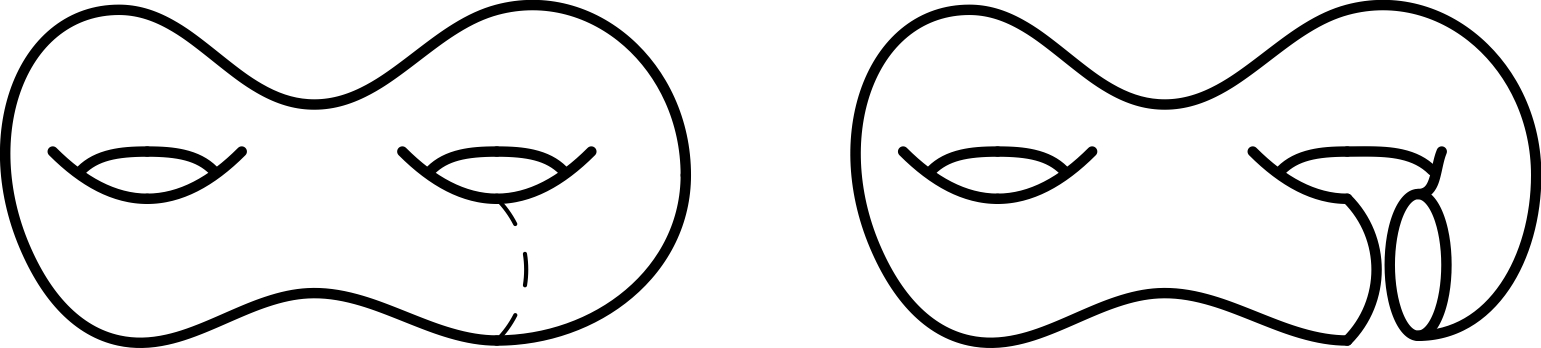
\includegraphics{PDF/cutopen.jpg}
 \caption{Cutting open a manifold by slicing along a closed
hypersurface (dashed) results in a manifold with boundary.}
 \label{cutopen}
 \end{figure}
%texpreamble
%("  \usepackage{amsmath}
% \usepackage[LY1]{fontenc}
% \usepackage[expert,LY1,mylucidascale]{mylucidabr}
% ");
%defaultpen(  fontcommand("\normalfont") + fontsize(10) ); 
%
%from graph access *;
%unitsize(0.4cm);
%
%pen thickpen = linewidth(1.25);
%
%currentpen = thickpen;
%
%void lefthalf(real x) {
%	draw( (x,0.5){W}..{NW}(x-1, 1) );
%	draw( (x,1){W}..{SW}(x-0.7, 0.8) );
%	}
%void righthalf(real x) {
%	draw( (x,0.5){E}..{NE}(x+1, 1) );
%	draw( (x,1){E}..{SE}(x+0.7, 0.8) );
%	}
%void hole(real x) {lefthalf(x); righthalf(x);}
%
%void M(real m){
%	draw( (m,-1){W}..(m-2,-0.5)..(m-4,-1)..(m-5,0)..(m-4,2.5)..(m-2,1.5)..(m,2.5)..{S}(m+2,0.75) );
%	hole(m-3.7);
%	}
%
%M(0); hole(0); draw( (2,0.75){S}..{W}(0,-1) ); 
%draw( (0,-1){NE}..(0,0.5){NW}, dashed );
%
%M(9); 
%draw( (9,-1){NE}..(9,0.5){NW} );
%draw( ellipse( (9.75,-0.2), 0.3, 0.75 ) );
%lefthalf(9);
%draw( (9,1){E}..{SE}(9.9, 0.8) );
%draw( (9.75,0.55){E}..{NNE}(10, 1) );
%draw( (11,0.75){S}..{W}(9.75, -0.95) );


The boundary of~$M'_1$
(namely, two copies of~$C_1$) is isometric to the boundary
of~$M'_2$ (namely, two copies of~$C_2$)
\csee{NonOrientDblCover}. So we may glue $M'_1$ and $M'_2$
together, by identifying $\bdry M'_1$ with~$\bdry M'_2$
\csee{hybridfig}, as described in the following
well-known proposition.

\begin{figure}[ht]
 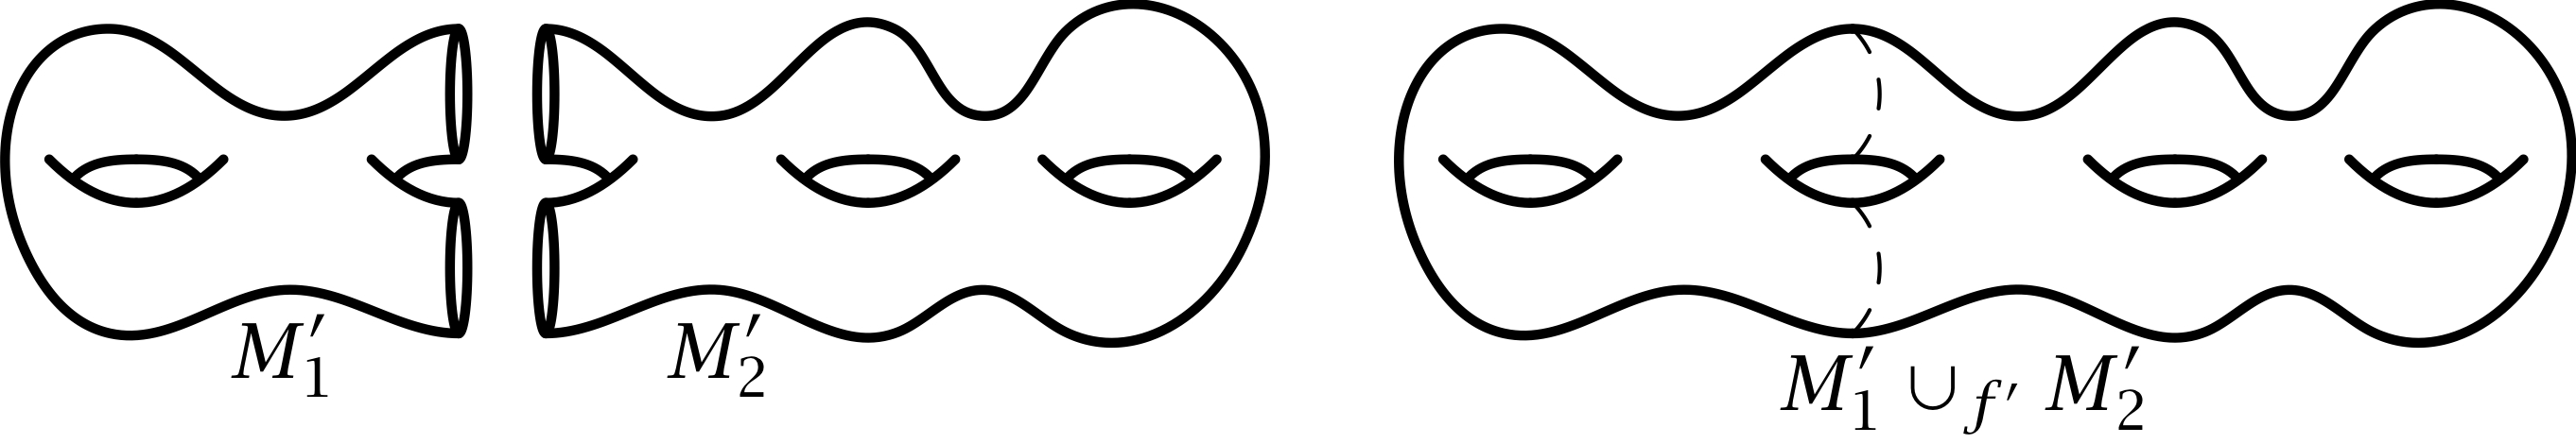
\includegraphics{PDF/hybrid.jpg}
 \caption{Gluing $M_1'$ to $M_2'$ along their boundaries
results in a manifold without boundary.}
 \label{hybridfig}
 \end{figure}
%texpreamble
%("  \usepackage{amsmath}
% \usepackage[LY1]{fontenc}
% \usepackage[expert,LY1,mylucidascale]{mylucidabr}
% ");
%defaultpen(  fontcommand("\normalfont") + fontsize(10) ); 
%
%from graph access *;
%unitsize(0.39cm);
%
%pen thickpen = linewidth(1.25);
%
%currentpen = thickpen;
%
%void lefthalf(real x) {
%	draw( (x,0.5){W}..{NW}(x-1, 1) );
%	draw( (x,1){W}..{SW}(x-0.7, 0.8) );
%	}
%void righthalf(real x) {
%	draw( (x,0.5){E}..{NE}(x+1, 1) );
%	draw( (x,1){E}..{SE}(x+0.7, 0.8) );
%	}
%void hole(real x) {lefthalf(x); righthalf(x);}
%
%void M(real m){
%	draw( (m,-1){W}..(m-2,-0.5)..(m-4,-1)..(m-5,0)..(m-4,2.5)..(m-2,1.5)..{E}(m,2.5) );
%	lefthalf(m);
%	hole(m-3.7);
%	}
%
%M(0);
%
%draw( ellipse( (0,-0.25), 0.1, 0.75 ) );
%draw( ellipse( (0,1.75), 0.1, 0.75 ) );
%
%void N(real n){
%	draw( (n,-1){E}..(n+2,-0.5)..(n+4,-1)..(n+5,-0.5)..(n+6,-1)..(n+8,0)
%		..(n+6,2.5)..(n+5,1.5)..(n+4,2.5)..(n+2,1.5)..{W}(n,2.5));
%	righthalf(n);
%	hole(n + 3.7);
%	hole(n + 6.7);
%	}
%N(1);
%draw( ellipse( (1,-0.25), 0.1, 0.75 ) );
%draw( ellipse( (1,1.75), 0.1, 0.75 ) );
%
%M(16); N(16);
%draw( (16,-1){NE}..{NW}(16,0.5) , dashed );
%draw( (16,1){NE}..{NW}(16,2.5) , dashed );
%
%label( "$M_1'$", (-2,-1.25) ); 
%label( "$M_2'$", (3,-1.25) ); 
%label( "$M_1' \cup_{f'} M_2'$", (17.3,-1.65) ); 

\begin{prop}
 Suppose 
 \begin{itemize}
 \item $M'_1$ and~$M'_2$ are connected $n$-manifolds with
boundary, and
 \item $f' \colon \bdry M'_1 \to \bdry M'_2$ is any
homeomorphism.
 \end{itemize}
 Define a topological space $M'_1 \cup_{f'} M'_2$, by gluing
$M'_1$ to~$M'_2$ along their boundaries:
 \begin{itemize}
 \item let $M'_1 \disjunion M'_2$ be the disjoint union
of~$M'_1$ and~$M'_2$,
 \item define an equivalence relation on $M'_1 \disjunion
M'_2$ by specifying that we have $m \sim f'(m)$, for every $m \in
\bdry M'_1$, and
 \item let $M'_1 \cup_{f'} M'_2 = (M'_1 \disjunion
M'_2)/\mathord{\sim}$ be the quotient of $M'_1 \disjunion
M'_2$ by this equivalence relation.
 \end{itemize}
 Then $M'_1 \cup_{f'} M'_2$ is an $n$-manifold
\textup(without boundary\textup).
 \end{prop}

\begin{cor}
 Suppose 
 \begin{itemize}
 \item $M_1$ and~$M_2$ are connected, orientable
$n$-manifolds,
 \item $C_j$ is a closed $(n-1)$-submanifold of~$M_j$, and
 \item $f \colon C_1 \to C_2$ is any homeomorphism.
 \end{itemize}
 Define $M_1 \#_f M_2 = M'_1 \cup_{f'} M'_2$, where
 \begin{itemize}
 \item $M'_j$ is the manifold with boundary that is obtained by
slicing $M_j$ open along~$C_j$, and
 \item $f' \colon \bdry M'_1 \to \bdry M'_2$ is
defined by $f'(c,k) = \bigl( f(c), k \bigr)$, under a
natural identification of~$\bdry M'_j$ with $C_j
\times \{1,2\}$.
 \end{itemize}
 Then $M_1 \#_f M_2$ is a \textup(connected\textup)
$n$-manifold \textup(without boundary\textup).

Furthermore, 
 \begin{enumerate}
 \item $M_1 \#_f M_2$ is compact if and only if both
$M_1$ and~$M_2$ are compact, and
 \item $M_1 \#_f M_2$ is connected if and only if either
$M_1 \smallsetminus C_1$ or~$M_2 \smallsetminus C_2$ is
connected.
 \end{enumerate}
 \end{cor}

\begin{terminology}
 Gromov and Piatetski-Shapiro \cite{GromovPS} call the
manifold $M_1 \#_f M_2$ a \defit[hybrid (of hyperbolic
manifolds)]{hybrid} of~$M_1$ and~$M_2$, and they call this
construction \defit[interbreeding hyperbolic
manifolds]{interbreeding}.
 \end{terminology}

Unfortunately, gluing two Riemannian manifolds together does
not always result in a Riemannian manifold (in any natural
way), even if the gluing map~$f$ is an isometry from~$\bdry
M'_1$ to~$\bdry M'_2$.

\begin{eg}
 Let $M'_1 = M'_2$ be the closed unit disk in~$\real^2$, and
let $f \colon \bdry M'_1 \to \bdry M'_2$ be the identity
map. Then $M'_1 \cup_f M'_2$ is homeomorphic to the
$2$-sphere~$S^2$. The Riemannian metrics on~$M'_1$
and~$M'_2$ are flat, so the resulting Riemannian metric
on~$S^2$ would also be flat. However, there is no flat
Riemannian metric on~$S^2$. (This follows, for example,
from the Gauss-Bonnet Theorem.) 
 \end{eg}

We can eliminate this problem by putting a restriction on
the hypersurface~$C_j$.

\begin{defn}
Let $M$ be a hyperbolic $n$-manifold. 
 A \defit[totally!geodesic hypersurface]{totally geodesic hypersurface} in~$M$ is a (closed, nonempty) connected
submanifold~$C$ of~$M$, such that, for each point~$c$
of~$C$, there are
 \begin{itemize}
 \item a neighborhood~$U$ of~$c$ in~$M$,
 \item a point~$x$ in $\hyperbolic^{n-1} = \{\, v \in
\hyperbolic^n \mid v_1 = 0 \,\}$,
 \item a neighborhood~$V$ of~$x$ in~$\hyperbolic^n$, and
 \item a Riemannian isometry $g \colon U \to V$, such that
$g(U \cap C) = V \cap \hyperbolic^{n-1}$.
 \end{itemize}
 \end{defn}

\begin{rem} \label{totgeod=Hn-1}
 If $C$ is a totally geodesic hypersurface in a hyperbolic
$n$-manifold of finite volume, then there are
 \begin{itemize}
 \item a lattice~$\Gamma$ in $\PO(1,n)$, and
 \item an isometry $f \colon M \to \Gamma \backslash
\hyperbolic^n$,
 \end{itemize}
 such that $f(C)$ is the image of $\hyperbolic^{n-1}$ in
$\Gamma \backslash \hyperbolic^n$.
 \end{rem}

\begin{prop} \label{M1cupM2hyper}
 If
 \begin{itemize}
 \item $M_1$ and~$M_2$ are hyperbolic $n$-manifolds,
 \item $C_j$ is a totally geodesic hypersurface in~$M_j$,
 \item $f \colon C_1 \to C_2$ is a Riemannian isometry, 
 and
 \item $M_1$ and~$M_2$ have finite volume,
 \end{itemize}
 then $M_1 \#_f M_2$ is a hyperbolic $n$-manifold of finite
volume.
 \end{prop}

\begin{proof}
 The main issue is to show that each point of $\bdry M'_1$
has a neighborhood~$U$ in $M'_1 \cup_{f'} M'_2$, such that
$U$~is isometric to an open subset of~$\hyperbolic^n$. This
is not difficult \csee{M1cupM2hyperEx}.

We have $\vol(M_1 \#_f M_2) = \vol(M_1) + \vol(M_2) <
\infty$.

If $M_1 \#_f M_2$ is compact, then it is obviously
complete. More generally, since $M'_1$ and~$M'_2$ are
complete, and their union is all of $M'_1 \cup_f M'_2$, it
seems rather obvious that every Cauchy sequence in $M'_1
\cup_f M'_2$ has a convergent subsequence. Hence, it
seems to be more-or-less obvious that $M'_1 \cup_f M'_2$ is
complete.

Unfortunately, if $M_1 \#_f M_2$ is not compact, then there
is a technical difficulty arising from the possibility
that, theoretically, the Riemannian isometry~$f$ may not be
an isometry with respect to the topological metrics that
$C_1$ and~$C_2$ inherit as submanifolds of $M_1$ and~$M_2$,
respectively. 
We will ignore this issue.
 \end{proof}

The following \lcnamecref{Hn-1=totgeod} describes how we will construct the
totally geodesic hypersurface~$C_j$.

\begin{lem} \label{Hn-1=totgeod}
 Suppose
 \begin{itemize}
 \item $\Gamma$ is a torsion-free lattice in\/
$\PO(1,n)^\circ$,
 \item $C$ is the image of\/~$\hyperbolic^{n-1}$ in\/ $\Gamma
\backslash \hyperbolic^n$,
 \item $\tau \colon \hyperbolic^n \to \hyperbolic^n$ is the
reflection across\/ $\hyperbolic^{n-1}$, so
	$$\tau(v_0,v_1,\ldots,v_n) =
(v_0,v_1,\ldots, v_{n-1}, -v_n) ,$$
 \item $\Gamma \cap \PO(1,n-1)$ is a lattice in\/
$\PO(1,n-1)$,
and
 \item $\Gamma$ is contained in a torsion-free lattice\/
$\Gamma'$ of\/ $\PO(1,n)^\circ$, such that\/ $\Gamma'$ is
normalized by~$\tau$.
 \end{itemize}
 Then $C$ is a totally geodesic hypersurface in\/ $\Gamma
\backslash \hyperbolic^n$, and $C$~has finite volume
\textup(as an $(n-1)$-manifold\textup).
 \end{lem}

\begin{proof}
 It is clear, from the definition of~$C$, that we need only
show $C$~is a (closed, embedded) submanifold of $\Gamma
\backslash \hyperbolic^n$.

Let $\Gamma_0 = \{\, \gamma \in \Gamma \mid
\gamma(\hyperbolic^{n-1}) = \hyperbolic^{n-1} \,\}$. (Then
$\Gamma \cap \PO(1,n-1)$ is a subgroup of index at most two
in~$\Gamma_0$.) 
 The natural map
 $$ \phi \colon \Gamma_0 \backslash \hyperbolic^{n-1} \to
\Gamma \backslash \hyperbolic^n$$
 is proper \ccf{LattInH->ProperMap}, so~$C$, being the
image of~$\phi$, is closed.

Because $\phi$ is obviously an immersion (and is a proper
map), all that remains is to show that $\phi$~is injective.
This follows from the assumption on~$\Gamma'$
\csee{Hn-1=totgeodPfinj}.
 \end{proof}



\subsection{Construction of nonarithmetic lattices}

The following theorem is the key to the construction of
nonarithmetic lattices. We postpone the proof until later
in the section \csee{ArithHybrid->Cup=M1Pf,HybridMfromM'}.

\begin{defn} \label{ArithHypMfldDefn}
 A hyperbolic $n$-manifold of finite volume is
\defit[arithmetic!hyperbolic manifold]{arithmetic} if the
corresponding lattice~$\Gamma$ in $\PO(1,n)$
\csee{HyperMfld<>lattice} is arithmetic. (Note that $\Gamma$
is well-defined, up to conjugacy
\csee{HyperMfld->UniqueLatt}, so this definition is
independent of the choice of~$\Gamma$.)
 \end{defn}

\begin{thm} \label{ArithHybrid->hybrid=M1}
 Suppose
 \noprelistbreak
 \begin{itemize}
 \item $M_1$ and~$M_2$ are hyperbolic $n$-manifolds,
 \item $C_j$ is a totally geodesic hypersurface in~$M_j$,
 \item $f \colon C_1 \to C_2$ is a Riemannian isometry,
 \item $M_1$ and~$M_2$ have finite volume \textup(as
$n$-manifolds\textup),
 \item $C_1$ and~$C_2$ have finite volume \textup(as
$(n-1)$-manifolds\textup),
 and
 \item each of $M_1 \smallsetminus C_1$ and $M_2
\smallsetminus C_2$ is connected.
 \end{itemize}
 If the hyperbolic manifold $M_1 \#_f M_2$ is
arithmetic, then $M_1 \#_f M_2$ is commensurable
to~$M_1$; that is, there are
 \begin{enumerate}
 \item a finite cover~$\widetilde{M}$ of $M_1 \cup_f M_2$,
and
 \item a finite cover~$\widetilde{M_1}$ of~$M_1$,
 \end{enumerate}
 such that $\widetilde{M}$ is isometric
to~$\widetilde{M_1}$.
 \end{thm}

\begin{cor} \label{ArithHybrid->M1=M2}
 In the situation of \cref{ArithHybrid->hybrid=M1},
 if the hyperbolic manifold $M_1 \#_f M_2$ is
arithmetic, then $M_1$ is commensurable to~$M_2$.
 \end{cor}

\begin{proof}
 From \cref{ArithHybrid->hybrid=M1}, we know that $M_1
\#_f M_2$ is commensurable to~$M_1$. By interchanging $M_1$
and~$M_2$, we see that $M_1 \#_f M_2$ is also commensurable
to~$M_2$. By transitivity, $M_1$ is commensurable to~$M_2$.
 \end{proof}

\begin{cor} \label{NonarithInSO1n}
 There exist nonarithmetic lattices\/
$\Gamma_\text{\upshape cpct}$ and\/~$\Gamma_\text{\upshape
non}$ in\/ $\SO(1,n)$, such that\/ $\Gamma_\text{\upshape
cpct}$ is cocompact, and\/ $\Gamma_\text{\upshape non}$ is
not cocompact.
 \end{cor}

\begin{proof}
 We construct only $\Gamma_\text{\upshape non}$. (See
\cref{CocpctNonarithInSO1n} for the construction
of~$\Gamma_\text{\upshape cpct}$, which is similar.)

Define quadratic forms $B_1(x)$ and~$B_2(x)$
on~$\rational^{n+1}$ by
 \begin{align*}
 B_1(x) &= x_0^2 - x_1^2 - x_2^2 - \cdots - x_{n-1}^2 - x_n^2 \\
 \intertext{and}
 B_2(x) &= x_0^2 - x_1^2 - x_2^2 - \cdots - x_{n-1}^2 - 2 x_n^2 
 . 
 \end{align*}
 Let
 \begin{itemize}
 \item $\Gamma_1 \approx \SO(B_1;\integer)$,
 \item $\Gamma_2 \approx h^{-1} \SO(B_2;\integer) h$, where
	$$h = \diag(1,1,\ldots,1,\sqrt{2}) \in \GL(n+1,\real) ,$$
 \item $M_j = \Gamma_j \backslash \hyperbolic^n$,
 \item $C_j$ be the image of $\hyperbolic^{n-1}$ in~$M_j$,
 and
 \item $\widehat\Gamma_j = \Gamma_j \cap \SO(1,n-1)$.
 \end{itemize}
 Then \cref{ArithSOn1F} tells us that $\Gamma_1$ and~$\Gamma_2$ are noncocompact
(arithmetic) lattices in $\SO(1,n)$.
By passing to finite-index subgroups, we may assume
$\Gamma_1$ and~$\Gamma_2$ are torsion free
\csee{torsionfree}. Therefore, $M_1$ and~$M_2$ are hyperbolic
$n$-manifolds of finite volume \csee{HyperMfld<>lattice}.

Because $\widehat\Gamma_j \approx \SO(1,n-1;\integer)$ is a
lattice in $\SO(1,n-1)$, and $\SO(B_j;\integer)$ is
normalized by the involution~$\tau$ of
\cref{Hn-1=totgeod}, we know $C_j$~is a totally
geodesic hypersurface in~$M_j$ that has finite volume
\csee{Hn-1=totgeod}.

Let us assume that $M_1 \smallsetminus C_1$ and $M_2
\smallsetminus C_2$ are connected. (See
\cref{NonarithInSO1nPf(notconn)} for a way around this
issue, or note that this hypothesis can be achieved by
passing to finite covers of~$M_1$ and~$M_2$.)

We know that $\widehat \Gamma_1 \approx \widehat \Gamma_2$ (since
both groups are commensurable to $\SO(1,n-1;\integer)$).
By taking a little bit of care in the choice of $\Gamma_1$
and~$\Gamma_2$, we may arrange that $\widehat \Gamma_1 = \widehat
\Gamma_2$ \csee{hybrid:Gamma1=Gamma2Ex}. Then 
 $$ C_1 \iso \widehat \Gamma_1 \backslash \hyperbolic^{n-1}
 =  \widehat \Gamma_2 \backslash \hyperbolic^{n-1}
 \iso C_2 ,$$
 so there is an isometry $f \colon C_1 \to C_2$.

If $n$~is odd, then $M_1$ is not commensurable to~$M_2$
\csee{Gamma=Gamma'(nodd)->disc}, so
\cref{ArithHybrid->M1=M2} implies that $M_1 \#_f M_2$
is not arithmetic; therefore, the corresponding
lattice~$\Gamma_\text{\upshape non}$ is not arithmetic
\csee{ArithHypMfldDefn}. When $n$~is even, an additional
argument is needed; see \cref{hybrid:nEvenNotArith}.
 \end{proof}



\subsection{Proof of \cref{ArithHybrid->hybrid=M1}}
 \label{ArithHybrid->Cup=M1Pf}

Let us recall the following lemma, which was proved in
\cref{IntZarDense->EqualEx}.

\begin{lem} \label{IntZarDense->Equal}
 If 
 \begin{itemize}
 \item $G$ has no compact factors,
 \item $\Gamma_1$ and~$\Gamma_2$ are arithmetic lattices
in~$G$, and
 \item $\Gamma_1 \cap \Gamma_2$ is Zariski dense in~$G$,
 \end{itemize}
 then $\Gamma_1$ is commensurable to~$\Gamma_2$.
 \end{lem}

\begin{defn}
 Let $M'$ be a Riemmanian $n$-manifold with boundary. We say
that $M'$~is a \defit[hyperbolic!manifold!with totally
geodesic boundary]{hyperbolic manifold with totally
geodesic boundary} if 
 \begin{enumerate}
 \item $M'$~is complete,
 \item each point of $M' \smallsetminus \bdry M'$ has a
neighborhood that is isometric to an open set
in~$\hyperbolic^n$, and
 \item for each point~$p$ of~$\bdry M'$, there are
 \begin{itemize}
 \item a neighborhood~$U$ of~$p$ in~$M'$,
 \item a point~$x$ in $\hyperbolic^{n-1} = \{\, v \in
\hyperbolic^n \mid v_1 = 0 \,\}$,
 \item a neighborhood~$V$ of~$x$ in~$\hyperbolic^n$, and
 \item an isometry $g \colon U \to V^+$, where 
 $$ V^+ = \{\, v \in V \mid v_1 \ge 0 \,\} .$$
 \end{itemize}
 (Note that $g(U \cap \bdry M') = V \cap
\hyperbolic^{n-1}$.)
 \end{enumerate}
 \end{defn}

The following is a generalization of
\cref{ArithHybrid->hybrid=M1}  \csee{HybridMfromM'}.

\begin{thm} \label{ArithHybrid->Cup=M1}
 Suppose
 \begin{itemize}
 \item $M_1$ and~$M_2$ are hyperbolic $n$-manifolds,
 \item $M_j'$ is a connected, $n$-dimensional submanifold
of~$M_j$ with totally geodesic boundary,
 \item $f' \colon \bdry M_1' \to \bdry M_2'$ is an isometry,
 \item $M_1$ and~$M_2$ have finite volume \textup(as
$n$-manifolds\textup),
 \item $\bdry M_j'$ has only finitely many components,
 and
 \item $\bdry M_1'$ and~$\bdry M_2'$ have finite volume
\textup(as $(n-1)$-manifolds\textup).
 \end{itemize}
 If the hyperbolic manifold $M_1' \cup_{f'} M_2'$ is
arithmetic, then $M_1' \cup_{f'} M_2'$ is commensurable
to~$M_1$.
 \end{thm}

\begin{proof}
 \ 
 \begin{itemize}
 \item Let $M = M_1' \cup_{f'} M_2'$.
 \item Write $M = \Gamma \backslash \hyperbolic^n$, for
some torsion-free lattice~$\Gamma$ in $\PO(1,n)$.
 \item Let $\phi \colon \hyperbolic^n \to M$ be the
resulting covering map.
 \item Let $B = \phi^{-1}(\bdry M_1')$. Because $M_1'$ has
totally geodesic boundary, we know that $B$~is a union of
disjoint hyperplanes. (That is, each component of~$B$ is of
the form $g(\hyperbolic^{n-1})$, for some $g \in
\Ortho(1,n)$.)
 \item Let $V$ be the closure of some connected component
of $\hyperbolic^n \smallsetminus B$ that contains a point
of $\phi^{-1}(M_1')$.
 \item Let 
 $$\Gamma'
 = \{\, \gamma \in \Gamma \mid \gamma V = V \,\}
 = \{\, \gamma \in \Gamma \mid \text{interior}(\gamma V \cap V) \neq \emptyset \,\} $$
 \csee{VTessellation}, so $M'_1 = \phi(V) \iso \Gamma'
\backslash V$.
 \end{itemize}

By definition, $V$~is an intersection of half-spaces, so it
is (hyperbolically) convex; hence, it is simply connected.
Therefore, $V$~is the universal cover of~$M_1'$, and
$\Gamma'$ can be identified with the fundamental group
of~$M_1'$.

Since $M'_1 \subseteq M_1$, we may define
$\Gamma_1,\phi_1,B_1,V_1,\Gamma_1'$ as above, but with
$M_1$ in the place of~$M$. From the uniqueness of the
universal cover of~$M_1'$, we know that there is an isometry
$\psi \colon V \to V_1$, and an isomorphism $\psi_* \colon
\Gamma' \to \Gamma_1'$, such that $\psi(\gamma v) =
\psi_*(\gamma) \, \psi(v)$, for all $\gamma \in \Gamma'$
and $v \in V$. Since~$\psi$ extends to an isometry
of~$\hyperbolic^n$, we may assume (after replacing
$\Gamma_1$ with $\psi^{-1} \Gamma_1 \psi$) that $V = V_1$
and $\psi_* = \Id$. Hence $\Gamma' = \Gamma_1' \subset
\Gamma \cap \Gamma_1$. It suffices to show (after replacing
$\Gamma$~by a conjugate subgroup) that the Zariski closure
of~$\Gamma'$ contains $\PO(1,n)^\circ$, for then
\cref{IntZarDense->Equal} implies $\Gamma$ is
commensurable to~$\Gamma_1$.

\begin{claim}
 We may assume that the Zariski closure of\/~$\Gamma'$
contains $\PO(1,n)^\circ$.
 \end{claim}
 We may assume $\hyperbolic^{n-1}$ is one of the connected
components of~$\bdry V$. Since $\bdry M_1'$ has finite
volume, this means that
 \begin{equation} \label{ArithHybridPf-BdryLatt}
 \mbox{$\Gamma' \cap \SO(1,n-1)$ is a lattice in
$\PO(1,n-1)$.}
 \end{equation}
 Let $\closure{\Gamma'}$~be the Zariski closure
of~$\Gamma'$. From \pref{ArithHybridPf-BdryLatt} and the
Borel Density Theorem \pref{BDT(Zardense)}, we know that
$\closure{\Gamma'}$~contains $\PO(1,n-1)^\circ$. Then,
since $\PO(1,n-1)^\circ$ is a maximal connected subgroup of
$\PO(1,n)$ \csee{MaxlInPO1n}, we may assume that
$\closure{\Gamma'}^\circ = \PO(1,n-1)^\circ$. (Otherwise,
the claim holds.) Because $\closure{\Gamma'}^\circ$ has
finite index in~$\closure{\Gamma'}$ \see{Zar->AlmConn}, this
implies that $\PO(1,n-1)^\circ$ contains a finite-index
subgroup of~$\Gamma'$. In fact, 
 \begin{equation} \label{ArithHybridPf-FinInd}
 \begin{matrix}
 \text{$\{\, \gamma \in \Gamma' \mid \gamma H = H \,\}$ has
finite index in $\Gamma'$,}
\\ \text{for every connected component~$H$
of~$\bdry V$} .
\end{matrix}
 \end{equation}
 This will lead to a contradiction.

\setcounter{case}{0}

\begin{case}
 Assume $\bdry V$ is connected.
 \end{case}
 We may assume $\bdry V = \hyperbolic^{n-1}$. Then, by
passing to a finite-index subgroup, we may assume that
$\Gamma' \subset \PO(1,n-1)$ \see{ArithHybridPf-FinInd}.
 Define $g \in \Isom(\hyperbolic^n)$ by
 $$g(v_1,v_2,\ldots,v_n) = (-v_1,v_2,\ldots,v_n) .$$
 Then
 \begin{itemize}
 \item $g$~centralizes~$\Gamma'$, and
 \item $\hyperbolic^n = V \cup g(V)$.
 \end{itemize}
  Since $\Gamma' \backslash V \iso M_1'$ has finite
volume, we know that $\Gamma' \backslash g(V)$ also has
finite volume. Therefore
 $$ \Gamma' \backslash \hyperbolic^n 
 = (\Gamma' \backslash V) \cup \bigl( \Gamma' \backslash
g(V) \bigr) $$
 has finite volume, so $\Gamma'$~is a lattice in
$\PO(1,n)$. But this contradicts the Borel Density Theorem
\pref{BDT(Zardense)} (since $\Gamma' \subset \PO(1,n-1)$).

\begin{case} \label{ArithHybrid->Cup=M1PfNotConn}
 Assume $\bdry V$ is not connected.
 \end{case}
 Let $H_1$ and~$H_2$ be two distinct connected components
of~$\bdry V$. Replacing
$\Gamma'$ by a finite-index subgroup, let us assume that
each of~$H_1$ and~$H_2$ is invariant under~$\Gamma'$
\see{ArithHybridPf-FinInd}.

 To simplify the argument, let us assume that $\bdry M_1'$
is compact, rather than merely that it has finite volume.
(See \cref{HybridWithNoncpctBdry} for the general
case.) Therefore, $\Gamma' \backslash H_1$ is compact, so there
is a compact subset~$C$ of~$H_1$, such that $\Gamma' C =
H_1$. Let 
 $$ \delta = \min \{\, \dist(c, H_2) \mid c \in C\,\} > 0
.$$
 Because $\Gamma'$ acts by isometries, we have $\delta =
\dist(H_1,H_2)$. Now, since $\hyperbolic^n$ is negatively
curved, there is a unique point~$p$ in~$H_1$, such that
$\dist(p,H_2) = \delta$. The uniqueness implies that $p$~is
fixed by every element of~$\Gamma'$. Since $\Gamma$ acts
freely on~$\hyperbolic^n$ (recall that it is a group of
deck transformations), we conclude that $\Gamma'$ is
trivial. This contradicts the fact that $\Gamma' \backslash
H_1$ is compact. (Note that $H_1 \iso \hyperbolic^{n-1}$ is
not compact.)
 \end{proof}

\begin{exercises}

\item \label{HyperMfld<>latticePfEx}
 Prove \cref{HyperMfld<>lattice}.

\item \label{HyperMfld->UniqueLatt}
 Show that if $\Gamma_1$ and~$\Gamma_2$ are torsion-free
lattices in $\PO(1,n)$, such that $\Gamma_1 \backslash
\hyperbolic^n$ is isometric to $\Gamma_2 \backslash
\hyperbolic^n$, then $\Gamma_1$ is conjugate to~$\Gamma_2$.
 \hint{Any isometry $\phi \colon \Gamma_1 \backslash
\hyperbolic^n \to \Gamma_2 \backslash \hyperbolic^n$ lifts
to an isometry of~$\hyperbolic^n$.}

 \item \label{NonOrientDblCover}
 Let $C$ be a closed, connected hypersurface in an
orientable Riemannian manifold~$M$, and let $M'$ be the
manifold with boundary that results from cutting~$M$ open,
by slicing along~$C$. Show:
 \begin{enumerate}
 \item If $C$~is orientable, then the boundary of~$M$ is
two copies of~$C$.
 \item If $C$ is not orientable, then the boundary is the
orientable double cover of~$C$.
 \item If $C$ is isometric to a closed, connected
hypersurface~$C_0$ in an orientable Riemannian
manifold~$M_0$, and $M'_0$ is the manifold with boundary
that results from cutting~$M_0$ open, by slicing
along~$C_0$, then the boundary of~$M'$ is isometric to the
boundary of~$M'_0$.
 \end{enumerate}

\item \label{M1cupM2hyperEx}
 For $M_1$, $M_2$, and~$f$ as in
\cref{M1cupM2hyperEx}, show that if $p \in \bdry
M'_1$, then $p$~has a neighborhood~$U$ in $M'_1 \cup_f
M'_2$, such that $U$~is isometric to an open subset
of~$\hyperbolic^n$.
 \hint{Find a ball~$V$ around a point~$x$
in~$\hyperbolic^{n-1}$, and isometries $g_1 \colon U_1 \to
V^+$ and $g_2 \colon U_2 \to V^-$, where $U_j$~is a
neighborhood of~$p$ in~$M'_j$, with $g_1|_{\bdry M'_1}
= (g_2 \circ f)|_{\bdry M'_1}$.}

\item \label{Hn-1=totgeodPfinj}
 For $\phi \colon \Gamma_0 \backslash
\hyperbolic^{n-1} \to \Gamma \backslash \hyperbolic^n$, as defined in the proof of \cref{Hn-1=totgeod}, show that $\phi$ is
injective.
 \hint{Suppose $\gamma x = y$, for some $\gamma \in \Gamma$
and $x,y \in \hyperbolic^{n-1}$. Then $\gamma^{-1} \tau
\gamma \tau$ is an element of~$\Gamma'$ that fixes~$x$, so
it is trivial. Hence, the fixed-point set of~$\tau$ is
$\gamma$-invariant.}

\item \label{CocpctNonarithInSO1n}
 Assume $n$~is odd, and construct a cocompact,
nonarithmetic lattice $\Gamma$ in $\SO(1,n)$.
 \hint{Let $F = \rational[\sqrt{2}]$, define $B_1(x) = \sqrt{2} x_0^2 - x_1^2 - x_2^2 - \cdots -
x_{n-1}^2 - x_n^2$
 and
 $B_2(x) = \sqrt{2} x_0^2 - x_1^2 - x_2^2 - \cdots -
x_{n-1}^2 - 3x_{n+1}^2$,
 and use the proof of \cref{NonarithInSO1n}.}

\item \label{hybrid(notconn)}
 In the notation of the proof of \cref{NonarithInSO1n},
assume that $M_1 \smallsetminus C_1$ and $M_2
\smallsetminus C_2$ are \emph{not} connected; let $M'_j$ be
the closure of a component of $M_j \smallsetminus C_j$.
Show that if $f' \colon C_1 \to C_j$ is any isometry (and
$n$~is odd), then $M'_1 \cup_{f'} M'_2$ is a
\emph{nonarithmetic} hyperbolic $n$-manifold of finite
volume.

\item \label{NonarithInSO1nPf(notconn)}
 Eliminate the assumption that $M_1 \smallsetminus C_1$ and
$M_2 \smallsetminus C_2$ are connected from the proof of
\cref{NonarithInSO1n}.
 \hint{Define
 $B_3(x) = x_0^2 - x_1^2 - x_2^2 - \cdots -
x_{n-1}^2 - 3
x_n^2$. If $M_j \smallsetminus C_j$ has the same number
of components as $M_k \smallsetminus C_k$ (and $j \neq k$),
then either \cref{hybrid(notconn)} or the proof of
\cref{NonarithInSO1n} applies.}

\item \label{hybrid:Gamma1=Gamma2Ex}
 For $B_1(x)$ and $B_2(x)$ as in the proof of
\cref{NonarithInSO1n}, show that there are finite-index
subgroups~$\Gamma_1$ and~$\Gamma_2$ of $\SO(B_1;\integer)$
and $\SO(B_2;\integer)$, respectively, such that
 \begin{enumerate}
 \item $\Gamma_1$ and~$\Gamma_2$ are torsion free, and
 \item $\Gamma_1 \cap \SO(1,n-1) = \Gamma_2 \cap
\SO(1,n-1)$.
 \end{enumerate}
 \hint{Let $\Gamma_j = \Lambda \cap \SO(B_j;\integer)$,
where $\Lambda$ is a torsion-free subgroup of finite index
in $\SL(n+1,\integer)$.}

\item \label{hybrid:nEvenNotArith}
 In the notation of the proof of \cref{NonarithInSO1n},
show that if $n$~is even (and $n \ge 4$), then
$\Gamma_\text{\upshape non}$ is not arithmetic.
 \hint{If $\Gamma_\text{\upshape non}$ is arithmetic, then
its intersection with $\SO(1,n-1)$ is arithmetic in
$\SO(1,n-1)$, and $n-1$ is odd.}

\item \label{HybridMfromM'}
 Derive \cref{ArithHybrid->hybrid=M1} as a corollary of
\cref{ArithHybrid->Cup=M1}.
 \hint{Apply \cref{ArithHybrid->Cup=M1} to
$\widetilde{M_j} = M_j \#_{f_j} M_j$, where $f_j \colon C_j
\to C_j$ is the identity map. Note that $\widetilde{M_j}$
is a double cover of~$M_j$, so $\widetilde{M_j}$ is
commensurable to~$M_j$.}

\item \label{VTessellation}
 For $\Gamma$ and~$V$ as in the proof of
\cref{ArithHybrid->Cup=M1}, let $\interior V$ be the
interior of~$V$, and show, for each $\gamma \in \Gamma$,
that if $\gamma \interior V \cap \interior V \neq \emptyset$,
then $\gamma \interior V = \interior V$.

\item \label{MaxlInPO1n}
 Show that if $H$ is a connected subgroup of $\PO(1,n)$
that contains $\PO(1,n-1)^\circ$, then $H =
\PO(1,n-1)^\circ$.

\item \label{HybridWithNoncpctBdry}
 Eliminate the assumption that $\bdry M_1'$ is compact from
\cref{ArithHybrid->Cup=M1PfNotConn} of the proof of
\cref{ArithHybrid->Cup=M1}.
 \hint{The original proof applies unless $\dist(H_1,H_2) =
0$, which would mean that $H_1$ and~$H_2$ intersect at
infinity. This intersection is a single point, and it is
invariant under~$\Gamma'$, which contradicts the Zariski
density of~$\Gamma'$.}

\end{exercises}





\section{Noncocompact arithmetic subgroups of \texorpdfstring{$\SL(3,\real)$}{SL(3,R)}}
\label{NonLattinSL3Sect}

We saw in \cref{NoncocpctSL2R=SL2Z} that
$\SL(2,\integer)$ is essentially the only noncocompact,
arithmetic subgroup of $\SL(2,\real)$. So it may be
surprising that $\SL(3,\integer)$ is \emph{not} the only
one in $\SL(3,\real)$.

\begin{prop} \label{NoncocpctInSL3Eg}
 Let
 \begin{itemize}
 \item $L$ be a real quadratic extension of\/~$\rational$, so
$L = \rational\bigl[\! \sqrt{r} \bigr]$, for some square-free positive
integer $r \ge 2$,
 \item $\sigma$ be the nontrivial Galois automorphism of~$L$,
 \item $\widetilde\sigma$ be the automorphism of\/ $\Mat_{3
\times 3}(L)$ induced by applying~$\sigma$ to each entry
of a matrix,
 \item $J_3 = 
 \begin{Smallbmatrix}
 0 & 0 & 1 \\
 0 & 1 & 0 \\
 1 & 0 & 0
 \end{Smallbmatrix}$,
 and
 \item $\Gamma = \SU \bigl( J_3, \sigma; \integer \bigl[\! \sqrt{r}
\bigr] \bigr)
 = 
 \bigset{
 g \in \SL \bigl( 3, \integer \bigl[\! \sqrt{r} \bigr] \bigr)
 }{
 \widetilde\sigma(g^{\transpose}) J_3 \, g = J_3
 }$.
 \end{itemize}
 Then:
 \begin{enumerate}
 \item \label{NoncocpctInSL3Eg-latt}
 $\Gamma$ is an arithmetic subgroup of\/ $\SL(3,\real)$,
 \item \label{NoncocpctInSL3Eg-noncocpct}
 $\Gamma$ is not cocompact, and
 \item \label{NoncocpctInSL3Eg-Qrank}
 no conjugate of\/~$\Gamma$ is commensurable to\/ $\SL(3,\integer)$.
% $\Qrank(\Gamma) = 1$.
 \end{enumerate}
 \end{prop}

\begin{proof}
 \pref{NoncocpctInSL3Eg-latt} This is a special case of
\cref{GFxR}\pref{FClassicalDefn-SUSL}, but we
provide a concrete, explicit proof (using the
methods of \cref{MakeArithLattSect,RestrictScalarsSect}).

Define
\noprelistbreak
 \begin{itemize}
 \item $\Delta \colon L^3 \to \real^6$ by $\Delta(v) =
\bigl( v,J_3 \, \sigma(v) \bigr)$,
 \item $V_{\rational} = \Delta(L^3)$,
 \item $\Zlatt = \Delta \bigl( \integer[\sqrt{r}]^3
\bigr)$, and
 \item $\rho \colon \SL(3,\real) \to \SL(6,\real)$ by
	$$ \text{$\rho(A)(v,w) = \bigl( Av, (A^T)^{-1}w \bigr)$ 
	\ for $v,w \in \real^3$} .$$
 \end{itemize}
 Then 
 \begin{itemize}
 \item $V_{\rational}$ is a $\rational$-form of~$\real^6$
\fullccf{Delta(O)=VSLatt}{F},
 \item $\Zlatt$ is a $\integer$-lattice
in~$V_{\rational}$ \fullccf{Delta(O)=VSLatt}{O},  
 \item $\rho$~is a homomorphism, 
 \item $\rho \bigl( \SL(3,\real) \bigr)$ is defined
over~$\rational$ (with respect to the
$\rational$-form~$V_{\rational}$)
(see \pref{NoncocpctInSL3Eg-/Q} below), % !!!
and
 \item $\Gamma = \{\, g \in \SL(3,\real) \mid \rho(g)
\Zlatt = \Zlatt \,\} $ \ccf{End(R4)Q}.
 \end{itemize}
 Hence, \fullcref{AbstractArith}{arith} (together with
\cref{arith->latt}) implies that $\Gamma$ is an
arithmetic subgroup of $\SL(3,\real)$.

Now let us show that 
 \begin{equation} \label{NoncocpctInSL3Eg-/Q}
 \mbox{$\rho \bigl( \SL(3,\real) \bigr)$ is defined
over~$\rational$.}
 \end{equation}
 This can be verified directly, by finding appropriate
$\rational$-polynomials, but let us, instead,
show that $\rho \bigl( \SL(3,\real) \bigr)_{\rational}$ is
dense in $\rho \bigl( \SL(3,\real) \bigr)$.

Define $U_1$ as in \eqref{NoncocpctInSL3EgPf-UGamma} below, % @@@
but allowing $a,b,c$ to range over all of~$\rational$, instead
of only~$2\integer$. Then $\rho(U_1) V_{\rational} \subset
V_{\rational}$ \csee{NoncocpctInSL3Ex-U1/Q}, so we have $\rho(U_1)
\subseteq \rho \bigl( \SL(3,\real) \bigr)_{\rational}$.
Furthermore, $U_1$ is dense in
 $$ U = 
 \begin{Smallbmatrix}
 1 & * & * \\
 0 & 1 & * \\
 0 & 0 & 1 
 \end{Smallbmatrix}
 .$$
 Similarly, there is a dense subgroup~$U_2$
of~$U^\transpose$, with $\rho(U_2) \subseteq \rho \bigl(
\SL(3,\real) \bigr)_{\rational}$
\csee{NoncocpctInSL3Ex-U2}. Since $\langle U, U^\transpose
\rangle = \SL(3,\real)$, we know that $\langle U_1,U_2
\rangle$ is dense in $\SL(3,\real)$, so $\rho \bigl(
\SL(3,\real) \bigr)_{\rational}$ is dense in $\rho \bigl(
\SL(3,\real) \bigr)$. Therefore $\rho \bigl( \SL(3,\real)
\bigr)$ is defined over~$\rational$ \see{QptsDense}.

\pref{NoncocpctInSL3Eg-noncocpct}
 By calculation, one may verify, directly from the
definition of~$\Gamma$, that the subgroup
 \begin{equation} \label{NoncocpctInSL3EgPf-UGamma}
 U_\Gamma = \bigset{
 \begin{bmatrix}
 1& a + b \sqrt{r} & -(a^2 - r b^2)/2 + c \sqrt{r} \\
 0& 1                 &  -a + b \sqrt{r} \\
 0& 0                 & 1 
 \end{bmatrix}
 } { a,b,c \in 2 \integer }
 \end{equation}
 is contained in~$\Gamma$. Then, since every element
of~$U_\Gamma$ is unipotent, it is obvious that $\Gamma$ has
nontrivial unipotent elements. So the Godement Criterion
\pref{GodementCriterion} implies that $G/\Gamma$
is not compact.

\pref{NoncocpctInSL3Eg-Qrank}
We sketch a proof. Choose an element $\omega \in \integer \bigl[ \sqrt{r} \bigr]$, such that $\sigma(\omega) = 1/\omega$. Then $\diag(\omega, 1, \omega^{-1})$ is a hyperbolic element of~$\Gamma$ that normalizes the maximal unipotent subgroup~$U_\Gamma$. On the other hand, it is easy to see that if $U'_\integer$ is any subgroup of $\SL(3,\integer)$ that is commensurable to the maximal unipotent subgroup $U_\integer$, then $U'_\integer$ has finite index in $\nzer_{\SL(3,\integer)}(U'_\integer)$. Since all of the maximal unipotent subgroups of $\SL(3,\integer)$ are conjugate (up to commensurability) under $\SL(3,\rational)$, this implies that  no conjugate of~$\Gamma$ is commensurable to $\SL(3,\integer)$.

Here is a more complete argument that is based on the notion of $\rational$-rank, which will be explained in \cref{QrankChap}.
 Define a nondegenerate $\sigma$-Hermitian form $B(x,y)$
on~$L^3$ by $B(x,y) = \sigma(x^\transpose) \, J_3 \, y$.
Then $v = (1,0,0)$ is an \term{isotropic vector} for~$B$ (i.e., $B(v,v) = 0$). On the other
hand, because $B$~is nondegenerate, the dimension of the orthogonal complement
of any subspace is equal to the codimension of the subspace.
Since $L^3$~is $3$-dimensional, this implies there is no 2-dimensional subspace that consists entirely of isotropic vectors. Therefore, $\Qrank \Gamma = 1$ \fullccf{QrankEg}{SOQ}. However, we have $\Qrank \SL(3,\integer) = 2$ \fullccf{QrankEg}{SL}. Two lattices with different $\rational$-ranks cannot be conjugate. (They cannot even be abstractly commensurable.)
 \end{proof}

\begin{rems} \ 
\noprelistbreak
 \begin{enumerate}
 \item From 
% Recall that $\Qrank \bigl( \SL(3,\integer) \bigr) =
%2$ (see~\ref{QrankIntroEgs} and~\fullref{QrankEg}{SL}).
%Therefore, 
\fullcref{NoncocpctInSL3Eg}{Qrank}, we know that none
of the arithmetic subgroups in \cref{NoncocpctInSL3Eg} are
conjugate to a subgroup that is commensurable to
$\SL(3,\integer)$. 

Indeed, let $X = \SL(3,\real)/\SO(3)$ be the symmetric space
associated to $\SL(3,\real)$. \Cref{HattoriThm}
implies that if $\Gamma$ is one of the arithmetic subgroups constructed
in \cref{NoncocpctInSL3Eg}, then the geometry of the
locally symmetric space $\Gamma \backslash X$ is very
different from that of $\SL(3,\integer) \backslash X$.
Namely, $\Gamma \backslash X$ is only mildly noncompact: it
merely has cusps, which means that its asymptotic cone is a
union of finitely many rays. In contrast, the asymptotic cone
of $\SL(3,\integer) \backslash X$ is a
2-complex, not just a union of rays. Even from a distance,
$\Gamma \backslash X$ and $\SL(3,\integer) \backslash X$
look completely different.

\item Different values of~$r$ always give essentially
different arithmetic subgroups \csee{GammaSL3R(r1<>r2)}, but this is
not so obvious.
 \end{enumerate}
 \end{rems}

The classification results in
\cref{ArithClassicalChap} imply that these are the
only arithmetic subgroups of $\SL(3,\real)$ that are not cocompact:

\begin{prop}[\csee{AllNoncocptSL3R}] \label{AllNoncocptSL3RStated}
 $\SL(3,\integer)$ and the arithmetic subgroups constructed in
\cref{NoncocpctInSL3Eg} are the only noncocompact
arithmetic subgroups of\/ $\SL(3,\real)$ \textup(up to
commensurability and conjugates\textup).
 \end{prop}

 

\begin{exercises}

\item \label{NoncocpctInSL3Ex-U1/Q}
 For $U_1$, $\rho$, and~$V_{\rational}$ as in the proof
of~\fullcref{NoncocpctInSL3Eg}{latt}, show that $\rho(U_1)
V_{\rational} \subseteq V_{\rational}$.

\item \label{NoncocpctInSL3Ex-U2}
 In the notation of the proof of
\cref{NoncocpctInSL3Eg}, find a dense subgroup~$U_2$
of 
 $$ \begin{Smallbmatrix}
 1 & 0 & 0 \\
 * & 1 & 0 \\
 * & * & 1 
 \end{Smallbmatrix} ,$$
 such that $\rho(U_2) \subseteq \rho \bigl( \SL(3,\real)
\bigr)_{\rational}$.

\item Assume the notation of the proof of
\cref{NoncocpctInSL3Eg}, and let $G = \rho \bigl(
\SL(3,\real) \bigr)$.
 \begin{enumerate}
 \item Show that $G$ is \defit[quasisplit $\rational$-form of
$G$]{quasisplit}. That is, show that some Borel subgroup of
$G$ is defined over~$\rational$.
 \item Show that every proper parabolic $\rational$-subgroup
of~$G$ is a Borel subgroup of~$G$.
 \end{enumerate}
 \hint{Let $B$ be the group of upper-triangular matrices in
$\SL(3,\real)$. Then $B$~is a Borel subgroup of
$\SL(3,\real)$, and $\rho(B)$ is defined over~$\rational$.}

\item \label{GammaSL3R(r1<>r2)}
 Let $\Gamma_1$ and~$\Gamma_2$ be noncocompact
arithmetic subgroups of $\SL(3,\real)$ that correspond to two different
values of~$r$, say~$r_1$ and~$r_2$. Show that $\Gamma_1$ is
not commensurable to any conjugate of~$\Gamma_2$.
 \hint{There is a diagonal matrix in~$\Gamma_1$ whose
trace is not in $\integer \bigl[\! \sqrt{r_2} \bigr]$.}

\end{exercises}










\section{Cocompact arithmetic subgroups of \texorpdfstring{$\SL(3,\real)$}{SL(3,R)}}\label{CocpctLattSL3R}

\Cref{SU2TotReal} used unitary groups over a totally real extension to construct cocompact, arithmetic subgroups of $\SL(2,\real)$. The same technique can be applied to $\SL(3,\real)$:

\begin{prop} \label{CocpctSL3RSU}
 Let
 \begin{itemize}
 \item $F$ be a totally real algebraic number field, such that $F \neq \rational$,
 \item $t,a,b \in F$, such that
 	\begin{itemize}
	\item $t, a, b > 0$,
	but
	\item $\sigma(t), \sigma(a), \sigma(b) < 0$ for every place $\sigma \neq \Id$,
	\end{itemize}
 \item $L = F \bigl[\! \sqrt{t}\bigr]$,
 \item $\tau$~be the Galois automorphism of~$L$ over~$F$,
 \item $\ints$ be the ring of integers of~$L$, and
 \item $\Gamma = \SU \bigl( \diag(a,b,-1), \tau ; \ints)$. 
 \end{itemize}
 Then $\Gamma$ is a cocompact, arithmetic subgroup of\/
$\SL(3,\real)$.
 \end{prop}

Here is a specific example:

\begin{cor} \label{EgCocpctUnitarySL3R}
Let 
	\begin{itemize}
	\item $t = \sqrt{2}$,
	\item $F = \rational \bigl[ t \bigr] = \rational \bigl[\! \sqrt{2} \bigr]$,
	\item $L = F \bigl[ \sqrt{t} \bigr] =  \rational \bigl[ \! \! \root 4 \of {2} \bigr]$,
	\item $\tau$ be the Galois automorphism of~$L$ over~$F$,
	\item $\ints \doteq \integer \bigl[ \! \! \root 4 \of {2}\bigr]$ be the ring of integers of~$L$,
	and
	\item $\Gamma = \SU( \Id_{3 \times 3}, \tau ; \ints )$.
	\end{itemize}
Then\/ $\Gamma$ is a cocompact, arithmetic subgroup of\/ $\SL(3,\real)$.
\end{cor}

 \begin{rem}
 It is necessary to assume $F \neq \rational$ in \cref{CocpctSL3RSU} (in other words, there is no analogue of \cref{SU2QCocpct} for $\SL(3,\real)$), because unitary groups over~$\rational$ yield only noncompact lattices in $\SL(3,\real)$ (as in \cref{NoncocpctInSL3Eg}), not cocompact ones \csee{SU3NotCocpct}.
 \end{rem}

Here is a quite different construction (not using unitary groups) that yields additional examples of cocompact, arithmetic subgroups. See
\cref{GoodLpForSL3Rcocpct} for explicit examples of~$L$
and~$p$ that satisfy the hypotheses.

\begin{prop} \label{CocpctSL3Rbands}
 Let
 \begin{itemize}
 \item $L$~be a cubic, Galois extension of~$\rational$
\textup(that is, a Galois extension of~$\rational$, such
that $|L:\rational| = 3$\textup),
 \item $\sigma$~be a generator of $\Gal(L/\rational)$
\textup(note that $\Gal(L/\rational)$, being of
order~$3$, is cyclic\textup),
 \item $\ints$ be the ring of integers of~$L$,
 \item $p \in \integer^+$,
 \item $\phi \colon L^3 \to \Mat_{3 \times 3}(L)$ be given
by
 \begin{equation} \label{embedDcyclic}
 \phi(x,y,z) =
 \begin{bmatrix}
 x & y & z \\
 p \, \sigma(z) & \sigma(x) & \sigma(y) \\
 p \, \sigma^2(y) & p \, \sigma^2(z) & \sigma^2(x)
 \end{bmatrix}
 ,
 \end{equation}
 and
 \item $\Gamma = \{\, \gamma \in \phi(\ints^3) \mid
\det \gamma = 1 \,\}$.
 \end{itemize}
 Then:
 \begin{enumerate}
 \item  \label{CocpctSL3Rbands-latt}
 $\Gamma$~is an arithmetic subgroup of\/ $\SL(3,\real)$.
 \item \label{CocpctSL3Rbands-cocpct}
 $\Gamma$ is cocompact if and only if $p \neq t \,
\sigma(t) \, \sigma^2(t)$, for all $t \in L$.
 \end{enumerate}
 \end{prop}

\begin{proof}
 \pref{CocpctSL3Rbands-latt} 
 It is easy to see that:
 \begin{itemize}
 \item $L \subset \real$ \csee{L/Qodd->LinR}.
 \item $\phi(L^3)$ and $\phi(\ints^3)$ are subrings
of $\Mat_{3 \times 3}(L)$ (even though $\phi$~is \emph{not}
a ring homomorphism).
 \item $\phi(L^3)$ is a $\rational$-form of $\Mat_{3 \times
3}(\real)$.
 \item $\phi(\ints^3)$ is a $\integer$-lattice in
$\phi(L^3)$.
 \item If we define $\rho \colon \Mat_{3 \times 3}(\real) \to
\End_{\real} \bigl( \Mat_{3 \times 3}(\real) \bigr)$ by
$\rho(g)(v) = gv$, then $\rho \bigl( \SL(3,\real) \bigr)$ is
defined over~$\rational$ (with respect to the
$\rational$-form $\phi(L^3)$ \csee{CocpctSL3RbandsEx/Q}).
 \item $\Gamma = \{\, g \in \SL(3,\real)
\mid g \, \phi(\ints^3) = \phi(\ints^3) \,\}$.
 \end{itemize}
 So $\Gamma$ is an arithmetic subgroup of $\SL(3,\real)$
\fullcsee{AbstractArith}{arith}.

(\ref{CocpctSL3Rbands-cocpct} $\Leftarrow$)
 If $\SL(3,\real)/\Gamma$ is not compact, then the Godement Criterion \pref{GodementCriterion} tells us there is a nontrivial
unipotent element~$u$ in~$\Gamma$. 
 This means $1$~is an eigenvalue of~$u$ (indeed, it is the
only eigenvalue of~$u$), so there is some nonzero $v
\in \real^3$ with $uv = v$. Hence $(u-1)v = 0$. Since $u
\neq \Id$ and $v \neq 0$, we conclude that $\phi(L^3)$ has a
nonzero element that is not invertible.

Hence, letting $D = \phi(L^3)$, it suffices to show that every nonzero element of $D$ is
invertible. (That is, $D$ is a
``division algebra\zz.'') For convenience, define $N \colon L \to
\rational$ by $N(t) = t \, \sigma(t) \, \sigma^2(t)$.
(In Algebraic Number Theory, $N$~is called the ``norm'' from~$L$ to~$\rational$.) We know that $p \neq N(t)$, for all
$t \in L$. It is easy to see that $N(t_1 t_2) = N(t_1) \,
N(t_2)$.
 
Note that if $xyz = 0$, but $(x,y,z) \neq (0,0,0)$, then
$\phi(x,y,z)$ is invertible. For example, if $z = 0$, then
$\det \phi(x,y,z) = N(x) + p\, N(y)$. Since $p \neq N(-x/y)
= -N(x)/N(y)$ (assuming $y \neq 0$), we see that $\det
\phi(x,y,z) \neq 0$, as desired. The other cases are
similar.

For any $x,y,z \in L$, with $z \neq 0$, we have
 $$ \phi \left( 1, - \frac{x}{p\, \sigma(z)}, 0 \right)
 \, \phi(x,y,z)
 = \phi(0,*,*)$$
 is invertible, so $\phi(x,y,z)$ is invertible.

(\ref{CocpctSL3Rbands-cocpct} $\Rightarrow$)
 If $p = t \, \sigma(t) \, \sigma^2(t)$, for some $t \in
L$, then $\phi(L^3) \iso \Mat_{3 \times
3}(\rational)$ \csee{phi(L3)=Mat}. 
From this, it is easy clear that
$\phi(\ints^3)$ contains nonidentity unipotent matrices. 
Since the determinant of any unipotent matrix is~$1$, these unipotents
belong to~$\Gamma$.
Therefore $\Gamma$ is not cocompact.
 \end{proof}


\begin{eg} \label{GoodLpForSL3Rcocpct}
 Let
 \begin{itemize}
 \item $\zeta = 2 \cos(2\pi/7)$,
 \item $L = \rational[\zeta]$, and
 \item $p$~be any prime that is congruent to either~$3$
or~$5$, modulo~$7$.
 \end{itemize}
 Then
 \begin{enumerate}
 \item $L$~is a cubic, Galois extension of~$\rational$, and
 \item $p \neq t \, \sigma(t) \, \sigma^2(t)$, for all $t
\in L$, and any generator~$\sigma$ of $\Gal(L/\rational)$.
 \end{enumerate}
 To see this, let $\omega = e^{2\pi i/7}$ be a primitive
$7^\text{th}$~root of unity, so $\zeta = \omega +
\omega^6$. Now it is well known that the Galois group of
$\rational[\omega]$ is cyclic of order~$6$, generated by
$\tau(\omega) = \omega^3$ \csee{Gal(cyclotomic)}. So the
fixed field~$L$ of $\tau^3$ is a cyclic extension of degree
$6/2 = 3$.

Now suppose $t \, \sigma(t) \, \sigma^2(t) = p$, for some
$t \in L^\times$. Clearing denominators, we have $s \,
\sigma(s) \, \sigma^2(s) = pm$, where
 \begin{itemize}
 \item $m \in \integer^+$,
 \item $s = a + b (\omega+\omega^6) + c
(\omega+\omega^6)^2$, with $a,b,c \in \integer$ and $p
\nmid \gcd(a,b,c)$.
 \end{itemize}
 Replacing~$\omega$ with the variable~$x$, we obtain
integral polynomials $s_1(x)$, $s_2(x)$, and~$s_3(x)$, such that 
 $$ s_1(x) s_2(x) s_3(x) = p m = 0 \mbox{ in }
 \frac{\integer_p[x]}{\langle x^6 + x^5 + \cdots + 1
\rangle}. $$
 This implies that $x^6 + x^5 + \cdots + 1$ is \emph{not}
irreducible in $\integer_p[x]$. This contradicts the choice
of~$p$ \csee{CycloqRedModp}.
 \end{eg}

\begin{rem} \label{AbelExtsAreCyclotomic}
 The famous \thmindex{Kronecker-Weber}{Kronecker-Weber Theorem} tells us that if $L$ is a Galois extension of~$\rational$, with abelian Galois group, then $L$ is contained in an extension obtained by adjoining an $n$th root of unity to~$\rational$ (for some~$n$). (\emph{Warning:} this does not hold for abelian extensions of algebraic number fields other than~$\rational$.) As a very special case, this implies that all of the cubic, Galois extension fields~$L$ of~$\rational$ can be
constructed quite explicitly, in the manner of \cref{GoodLpForSL3Rcocpct}:
 \begin{itemize}
 \item Choose $n \in \integer^+$, such that $\varphi(n)$ is
divisible by~$3$ (where 
 $$\varphi(n) = \# \{\, k \mid 1 \le k \le n, \ \gcd(k,n) =
1 \,\} $$
 is the Euler $\varphi$-function).
 \item Let $\omega = e^{2\pi i/n}$ be a primitive
$n^\text{th}$~root of unity.
 \item Let $H$ be any subgroup of index~$3$ in the
multiplicative group $(\integer_n)^\times$ of units
modulo~$n$.
 \item Let $\zeta = \sum_{k \in H} \omega^k = \sum_{k \in
H} \cos(2 \pi k/n)$.
 \item Let $L = \rational[\zeta]$.
 \end{itemize}
 \end{rem}

We have now seen that cocompact arithmetic subgroups of $\SL(3,\real)$ can be constructed
by two different methods: some are constructed by using unitary groups (as in \cref{CocpctSL3RSU}) and others are constructed by using ``division 
algebras'' $D = \phi(L^3)$ (as in \cref{DCocpctinSL3R}). We will see in the following % @@@
section that these two methods can be
combined: some cocompact arithmetic subgroups are constructed by using \emph{both}
unitary groups \emph{and} division algebras. The classification results in
\cref{QFormsOfSLnSect} show that all
cocompact arithmetic subgroups of $\SL(3,\real)$ can be obtained from these methods, using either unitary groups, division algebras, or 
a combination of the two (perhaps also combined with restriction of scalars). The same is true for the cocompact arithmetic subgroups of any $\SL(n,\real)$, with $n \ge 3$.

%\begin{prop} \label{CocpctSL3R}
% The arithmetic subgroups constructed in \cref{CocpctSL3RSU,CocpctSL3Rbands} are the only cocompact arithmetic subgroups
%in $\SL(3,\real)$ \textup(up to commensurability and
%conjugates\textup).
% \end{prop}

\begin{exercises}

\item \label{SU3NotCocpct}
Assume the situation of \cref{CocpctSL3RSU}, except that $F = \rational$.
More precisely, let 
	\begin{itemize}
	\item $a,b,c \in \rational$ (all nonzero),
	\item $L$ be a real quadratic extension of~$\rational$,
	\item $\tau$ be the Galois automorphism of~$L$ over~$\rational$,
	\item $\ints$ be the ring of integers of~$L$,
	\item $A = \diag( a,b,c )$,
	and
	\item $\Gamma = \SU ( A, \tau ; \ints )$, so $\Gamma$ is an arithmetic subgroup of\/ $\SL(3,\real)$.
	\end{itemize}
Show that $\Gamma$ is \underline{not} cocompact.
\hint{The equation $\tau( x{}^\transpose) A  x = 0$ for $ x \in L^3$ can be considered as an equation in $6$ variables over~$\rational$, so the Number Theory fact mentioned in the proof of \cref{NonCocptArithSOn1} implies it has a nontrivial solution.}

\item \label{L/Qodd->LinR}
 Let $L$~be a Galois extension of~$\rational$\,,
with $|L:\rational|$ odd. Show $L \subset \real$.

\item \label{CocpctSL3RbandsEx/Q}
 Assume the notation of the proof of
\cref{CocpctSL3Rbands}. For $h \in L^3$, define $T_h
\in \End_{\real} \bigl( \Mat_{3 \times 3}(\real) \bigr)$ by
$T_h(v) = \phi(h) \, v$.
 \begin{enumerate}
 \item Show that $\phi(h) \in \End_{\real} \bigl( \Mat_{3
\times 3}(\real) \bigr)_{\rational}$, where the $\rational$-form is  induced by the $\rational$-form
$\phi(L^3)$ of $\Mat_{3 \times 3}(\real)$. 
\hint{Show $\phi(h) \, \phi(L^3) \subseteq \phi(L^3)$.}
 \item Show that $\rho \bigl( \Mat_{3 \times 3}(\real)
\bigr)$ is the centralizer of $\{\, T_h \mid h \in L^3
\,\}$.
 \item Show that $\rho \bigl( \SL(3,\real) \bigr)$ is
defined over~$\rational$.
 \end{enumerate}

\item In the notation of \cref{CocpctSL3Rbands}, show
that if $p = t \, \sigma(t) \, \sigma^2(t)$, then the element 
$\phi\Bigl( 1,1/t, 1/ \bigl(t \, \sigma(t) \bigr) \Bigr)$ of $\phi(L^3)$ is not invertible.

\item \label{phi(L3)=Mat}
In the notation of \cref{CocpctSL3Rbands}, show that if 
$p = t \, \sigma(t) \, \sigma^2(t)$, for some $t \in
L$, then $\phi(L^3) \iso \Mat_{3 \times 3}(\rational)$.
\hint{$\bigl\{ \bigl( a, t \sigma(a), t \sigma(t) \sigma^2(a) \bigr) \bigr\}$
is a $3$-dimensional, $\phi(L)$-invariant $\rational$-subspace of~$L^3$.}

\item \label{CycloqRedModp}
 Let $p$ and~$q$ be distinct primes, and
 $$f(x) = x^{q-1} + \cdots + x + 1 .$$
 Show that $f(x)$ is reducible over~$\integer_p$ if and
only if there exists $r \in \{1,2,\ldots, q-2\}$, such that
$p^r \equiv 1 \pmod{q}$.
 \hint{Let $g(x)$ be an irreducible factor of $f(x)$, and
let $r = \deg g(x) < q-1$. Then $f(x)$ has a root~$\alpha$
in a finite field~$F$ of order~$p^r$. Since $\alpha$ is an
element of order~$q$ in~$F^\times$, we must have $q \mid \#
F^\times$.}

\end{exercises}










\section{Arithmetic subgroups of \texorpdfstring{$\SL(\lowercase{n},\real)$}{SL(n,R)}} \label{LattSlnRSect}

We will briefly explain how the previous results on $\SL(3,\real)$
can be generalized to higher dimensions. (The group $\SL(2,\real)$
is a special case that does not fit into this pattern.)
The proofs are similar to those for $\SL(3,\real)$.

In \cref{QuaternionAlgSect}, and in the proof of \cref{CocpctSL3Rbands}, we have seen that cocompact arithmetic subgroups of $\SL(n,\real)$ can sometimes be constructed by using rings in which every nonzero element has a multiplicative inverse. More such ``division algebras'' will be needed in order to construct all the arithmetic subgroups of $\SL(n,\real)$ with $n > 3$. 

%The list of classical Lie groups includes the groups
%$\SL(n,\quaternion)$ and $\SO(n,\quaternion)$, that are based on the ring of
%quaternions, which is a division algebra over~$\real$.
%Analogously, we have seen in \cref{EgArithGrpsChap} that $\rational$-forms are sometimes based on division algebras over~$\rational$. In fact, because $\rational$-forms can come from Restriction of Scalars \pref{ResScal->Latt}, the study of arithmetic groups involves division algebras not only over~$\rational$, but over extension fields of~$\rational$.
%In this section, we provide some basic information
%on division algebras and the associated unitary
%groups. Usually (but, unfortunately, not for $\SL(n,\real)$), it suffices to have some
%familiarity with the special case of quaternion algebras $\quaternion^{a,b}_F$
%\csee{QuaternionDefn}. 
%The
%interested reader can find a more substantial introduction to
%the theory of central division algebras (including how to
%construct them) in \cref{DivAlgsChap}. 


\subsection{Division algebras}

\begin{defn} \label{DivAlgDefn}
 An associative ring~$D$ is a \defit{division
algebra} over a field~$F$ if%
\noprelistbreak
 \begin{enumerate}
 \item \label{DivAlgDefn-F}
 $D$ contains~$F$ in its center 
 	(that is, $xf = fx$ for all $x \in D$ and $f \in F$),
 \item \label{DivAlgDefn-1}
 the element $1 \in F$ is the identity element of~$D$,
 \item \label{DivAlgDefn-dim}
 $D$ is finite-dimensional as a vector space over~$F$,
 and
 \item \label{DivAlgDefn-inv}
 every nonzero element of~$D$ has a multiplicative
inverse.
 \end{enumerate}
Furthermore, it is \defit[division algebra!central]{central} over~$F$ if the entire center of~$D$ is precisely~$F$.
 \end{defn}

\begin{rems} \ 
\noprelistbreak
 \begin{enumerate}
 \item $D$ is an \emph{algebra} over~$F$ if
\pref{DivAlgDefn-F} and~\pref{DivAlgDefn-1} hold. 
% \item The word \emph{central} requires the center of~$D$ to
%be exactly~$F$, not some larger field.
  \item The word \emph{division} requires
\pref{DivAlgDefn-inv}.
We also assume \pref{DivAlgDefn-dim}, although not all authors require this.
% \item We consider only associative algebras here, but the
%algebra of \term{octonions}, which
%is nonassociative, also arises in the theory of arithmetic
%groups \cf{Rrank1list}.
 \end{enumerate}
 \end{rems}

\begin{terminology}
 Division algebras are also called \defit[skew field]{skew fields}.
 	% or \defit[division ring]{division rings}.
 \end{terminology}

\begin{egs} \label{DivAlgEgs} \ 
\noprelistbreak
 \begin{enumerate}
 \item Any extension field of~$F$ is a division algebra over~$F$ (but is not usually central).
 \item \label{DivAlgEgs-H}
 $\quaternion = \quaternion^{-1,-1}_\real$ is a central division algebra over~$\real$.
 \item \label{DivAlgEgs-quat}
 More generally, a quaternion algebra $\quaternion^{a,b}_F$ is a
central division algebra over~$F$ if and only if $\Nred(x) \neq 0$,
for every nonzero $x \in \quaternion^{a,b}_F$
\csee{QuatInverses}.
 Note that this is consistent with \pref{DivAlgEgs-H}.
 \end{enumerate}
 \end{egs}

The following famous theorem shows that division algebras are the building blocks of simple algebras:

\begin{thm}[(\thmindex{Wedderburn's}Wedderburn's Theorem)] \label{WedderburnThm}
Let $A$ be a finite-dimensional algebra over a field~$F$. If $A$ is \defit[simple!ring]{simple} \textup(that is, if $A$ has no nonzero, proper, two-sided ideals\textup), then $A \iso \Mat_{n \times n}(D)$, for some~$n$ and some division algebra~$D$ over~$F$.
\end{thm}

\begin{proof}
Since $A$ is finite-dimensional, we may let $I$ be a minimal left ideal. 
Then $I$ is a left $A$-module that is \defit[simple!module]{simple} (that is, has no nonzero, proper submodules). So $\End_A(I)$ is a division algebra \csee{SchursLemma}; call it~$D$. 

We have $IA = A$, since $IA$ is a $2$-sided ideal and $A$~is simple. Hence, the minimality of~$I$ implies $A = Ia_1 \oplus \cdots \oplus Ia_n$, for some $a_1,\ldots,a_n \in A$ \csee{DirSumIdeals}. 

For $A$ considered as a left $A$-module, it is easy to see that each element of $\End_A(A)$ is multiplication on the right by an element of~$A$ \csee{End(A)=A}; therefore $\End_A(A) \iso A$.
On the other hand, it is easy to see that $Ia_i$ is isomorphic to~$I$ as a left $A$-module \csee{Ia=I}, so we have
	\begin{align*}
	\End_A(A) 
	&= \End_A(Ia_1 \oplus \cdots \oplus Ia_n)
	\iso \End_A(I^n)
	\\&\iso \Mat_{n \times n} \bigl( \End_A(I) \bigr)
	= \Mat_{n \times n}(D) 
	.  \end{align*}
Therefore $A \iso \Mat_{n \times n}(D) $.
%If we let $n = \dim_D(A)$, then the action of $A$ on~$I$ provides a homomorphism $A \to \Mat_{n \times n}(D)$. The homomorphism is injective (because its kernel must be trivial, since $A$ is simple). 
%The hard part (which we omit) is to show that the homomorphism is surjective; this  assertion is known as the \emph{\thmindex{Jacobson Density}{Jacobson Density Theorem}}.
\end{proof}

\begin{cor}
If $D$ is a central division algebra over~$F$, then we have $\dim_F D = d^2$, for some $d \in \integer^+$. \textup(This integer~$d$ is called the \defit[degree!of a division algebra]{\textit{degree}} of~$D$ over~$F$.\textup)
\end{cor}

\begin{proof}
Let $\overline{F}$ be the algebraic closure of~$F$. Then (from {Wedderburn's Theorem}), we see that $D \otimes_F \overline{F} \iso \Mat_{d \times d}(D')$, for some~$d$ and some central division algebra~$D'$ over~$\overline{F}$. Since $\overline{F}$ is algebraically closed, we must have $D' = \overline{F}$ \csee{DivAlg/AlgClosed}, so
	\begin{align*}
	\dim_F D = \dim_{\overline{F}} (D \otimes_F \overline{F})
	= \dim_{\overline{F}} \Mat_{d \times d}(\overline{F})
	= d^2 
	. & \qedhere \end{align*}
\end{proof}

In order to produce arithmetic groups from division algebras, the following \lcnamecref{OinDivAlg} provides an analogue of the ring of integers in an
algebraic number field~$F$. 

\begin{lem} \label{OinDivAlg}
 If $D$ is a division algebra over an algebraic
number field~$F$, then there is a subring~$\ints_D$
of~$D$, such that $\ints_D$ is a $\integer$-lattice
in~$D$. Any such subring is called an {\upshape\defit[order (in an algebraic number field)]{order}} in~$D$.
 \end{lem}

\begin{proof}
 Let $\{v_0,v_1,\ldots,v_r\}$ be a basis of~$D$
over~$\rational$, with $v_0 = 1$. Let
$\{c_{j,k}^\ell\}_{j,k,\ell=0}^r$ be the structure constants
of~$D$ with respect to this basis. That is, for $j,k \in
\{0,\ldots,r\}$, we have
 $ v_j v_k = \sum_{\ell=0}^r c_{j,k}^\ell v_\ell $.
 There is some nonzero $m \in \integer$, such that $m
c_{j,k}^\ell \in \integer$, for all $j,k,\ell$. Let
$\ints_D$ be the $\integer$-span of
$\{1, mv_1,\ldots,mv_r\}$.
 \end{proof}

In the proof of \cref{CocpctSL3Rbands}, we showed that
$\phi(L^3)$ is a division algebra if
 $p \neq t\, \sigma(t) \, \sigma^2(t)$.
 Conversely, it is known that every division algebra of degree~$3$ arises from the above construction. (In the terminology of ring theory, this means that every central division algebra of degree~$3$ is ``\label{CubicAlgIsCyclic}\term[division algebra!cyclic]{cyclic}\zz.'') Therefore, we can restate the \lcnamecref{CocpctSL3Rbands} in the following more abstract form.  
 
\begin{prop} \label{DCocpctinSL3R}
 Let
 \begin{itemize}
 \item $L$~be a cubic, Galois extension of\/~$\rational$,
 \item $D$ be a central division algebra of degree\/~$3$
over\/~$\rational$, such that $D$~contains~$L$ as a subfield,
and
 \item $\ints_D$ be an order in~$D$ \csee{OinDivAlg}.
 \end{itemize}
 Then there is an embedding $\phi \colon D \to \Mat_{3
\times 3}(\real)$, such that 
 \begin{enumerate}
 \item $\phi \bigl( \SL(1,D) \bigr)$ is a\/ $\rational$-form
of\/ $\Mat_{3 \times 3}(\real)$, and
 \item \label{DCocpctinSL3R-cocpct}
 $\phi \bigl( \SL(1,\ints_D) \bigr)$ is a cocompact,
arithmetic subgroup of\/ $\SL(3,\real)$.
 \end{enumerate}

Furthermore, $\phi \bigl( \SL(1,\ints_D) \bigr)$ is
essentially independent of the choice of~$\ints_D$ or
of the embedding~$\phi$. Namely, if $\ints_D'$
and~$\phi'$ are some other choices, then there is an
automorphism~$\alpha$ of\/ $\SL(3,\real)$, such that
$\alpha \phi' \bigl( \SL(1,\ints_D') \bigr)$ is
commensurable to $\phi \bigl( \SL(1,\ints_D)
\bigr)$.
 \end{prop}

This generalizes in an obvious
way to provide cocompact, arithmetic subgroups of
$\SL(n,\real)$. By replacing $\SL(1,\ints_D)$ with the
more general $\SL(m,\ints_D)$, we can also obtain arithmetic subgroups
that are not cocompact (if $n$ is not prime).

\begin{prop} \label{LattSLnRDivAlg}
 Let
 \noprelistbreak
 \begin{itemize}
 \item $D$ be a central division algebra of degree~$d$
over\/~$\rational$, such that $D$~splits over\/~$\real$,
 \item $m \in \integer^+$, and
 \item $\ints_D$ be $\integer$-lattice in~$D$ that is
also a subring of~$D$.
 \end{itemize}
 Then $\phi \bigl( \SL(m,\ints_D) \bigr)$ is an
arithmetic subgroup of\/ $\SL(dm,\real)$, for any embedding
$\phi \colon D \to \Mat_{d \times d}(\real)$, such that
$\phi(D)$ is a\/ $\rational$-form of\/ $\Mat_{d \times
d}(\real)$.

It is cocompact if and only if $m = 1$.
 \end{prop}



\subsection{Unitary groups over division algebras}
The definition of a unitary group is based on the Galois automorphism of a quadratic extension. This is a field automorphism of order~$2$. The following analogue makes it possible to define unitary groups over division algebras that are not required to be fields.

\begin{defn}
 Let $D$ be a central division algebra. A map $\tau
\colon D \to D$ is an \defit{anti-involution} if $\tau^2 =
\Id$ and $\tau$ is an \textbf{anti}-automorphism; that is,
$\tau(x+y) = \tau(x) + \tau(y)$ and $\tau(xy) =
\tau(y) \, \tau(x)$. (Note that $\tau$ reverses the order of
the factors in a product.)
 \end{defn}

\begin{terminology}
 Some authors call $\tau$ an involution, rather than an
anti-involution, but, to avoid confusion, our terminology emphasizes
the fact that $\tau$ is \emph{not} an automorphism (unless
$D$~is commutative).
 \end{terminology}

\begin{egs} \label{QuatConjRevDefn}
 Let $D$ be a quaternion division algebra. Then:
 \noprelistbreak
 \begin{enumerate}
 \item The map 
 \nindex{$\tau_c$ = conjugation on quaternion algebra}$\tau_c \colon D \to D$ defined by 
 $$\tau_c(a + bi + cj + dk) = a - bi - cj - dk$$
 is an anti-involution. It is called the \defit[anti-involution!standard]{standard
anti-involution} of~$D$, or the \defit[conjugation on
quaternion algebra]{conjugation} on~$D$, so $\tau_c(x)$ can also be denoted~$\overline{x}$.
 \item The map 
  \nindex{$\tau_r$ = reversion anti-involution on quaternion algebra}$\tau_r \colon D \to D$ defined by 
 $$\tau_r(a + bi + cj + dk) = a + bi - cj + dk$$
 is an anti-involution. It is called the
\defit[reversion anti-involution]{reversion} on~$D$.
 \end{enumerate}
 \end{egs}

\begin{defns} \label{SUDDefn}
Let $\tau$ be an anti-involution of a division
algebra~$D$ over~$F$. 
\noprelistbreak
 \begin{enumerate}
 \item A matrix $A \in \Mat_{n \times n}(D)$ is said to be \defit[Hermitian!matrix]{Hermitian} (or,
more precisely, \emph{$\tau$-Hermitian}) if $(A^\tau)^\transpose = A$.
\item Given a Hermitian matrix~$A$, we let
	$$ \SU(A,\tau; D) = \{\, g \in \SL(n,D) \mid (A^\tau)^\transpose A g = A \,\} .$$
 \end{enumerate}
 \end{defns}

%\begin{defn} \ 
%\noprelistbreak
% \begin{enumerate}
% \item Let $\tau$ be an anti-involution of a division
%algebra~$D$ over~$F$. A \defit{Hermitian form} (or,
%more precisely, a \emph{$\tau$-Hermitian form}) on~$D^n$ is a
%map $B \colon D^n \times D^n \to D$, such that
% \begin{itemize}
% \item $B(x_1 + x_2, y) = B(x_1,y) + B(x_2,y)$ and
% $B(x,y_1 + y_2) = B(x,y_1) + B(x,y_2)$, for all
%$x,x_1,x_2,y,y_1,y_2 \in D^n$, 
% \item $B(ax,y) = a B(x,y)$ and $B(x,ay) = B(x,y) \, \tau(a)$
%for all $a \in D$ and $x,y \in D^n$, and
% \item $B(y,x) = \tau \bigl( B(x,y) \bigr)$ for all $x,y
%\in D^n$.
% \end{itemize}
% \item The Hermitian form~$B$ is
%\defit[nondegenerate Hermitian form]{nondegenerate} if, for
%each nonzero $x \in D^n$, there exists $y \in D^n$, such that
%$B(x,y) \neq 0$.
% \end{enumerate}
% \end{defn}

%\begin{defn}
% Suppose $D$ is a central division algebra over a field~$F$,
%and $L$~is some extension field of~$F$. We say that
%$D$~\defit[splits over a field]{splits} over~$L$ if $D
%\otimes_F L \iso \Mat_{d \times d}(L)$, for some natural
%number~$d$. In this case, we call~$d$ the \defit[degree!of
%a division algebra)]{degree} of~$D$, and we have
%$\dim_F D = d^2$ (because $\dim_L (D \otimes_F L) = d^2$).
% \end{defn}
%
%Every central division algebra splits over some extension
%of~$F$:
%
%\begin{prop} \label{DxC=Mat}
% If $D$ is a central division algebra over a subfield~$F$
%of~$\complex$, then $D$~splits over~$\complex$.
% \end{prop}
%
%In fact, $D$ splits over a much smaller field
%than~$\complex$ (unless $F$~itself is almost all
%of~$\complex$).
%
%\begin{prop} \label{MaxFldSplits}
% If $D$ is a central division algebra over a field~$F$, and
%$L$~is any maximal subfield of~$D$, then $D$~splits over~$L$.
% \end{prop}
%
%\begin{proof}
% Define a ring homomorphism $f \colon D \otimes_F D \to
%\End_F(D)$ by $f(x,y)(v) = xvy$. Because $D$ is a division
%algebra, it is obvious that $D$~is an irreducible module for
%$f(1 \otimes D)$, so $D$~is irreducible for $f(L \otimes_F
%D)$.  Therefore, the Jacobson Density Theorem \pref{JacDensThm}
%implies that $f(L \otimes_F D)$ is isomorphic to $\Mat_{d
%\times d}(E)$, where 
% $$ E = \End_{f(L \otimes_F D)}(D) = f(L \otimes 1) \iso L $$
% \csee{C(MaxFld)}. Since $L \otimes_F D$ is simple
%\csee{AxBsimplealg}, we know that $f$~is faithful, so $L
%\otimes_F D \iso f(L \otimes_F D)$.
% \end{proof}

This notation makes it possible to state a version of \cref{CocpctSL3RSU} that
replaces the quadratic extension~$L$ with a larger division algebra.

\begin{prop} \label{LattSLnRSU}
 Let
 \begin{itemize}
 \item $L$ be a real quadratic extension of\/~$\rational$,
 \item $D$~be a central simple division algebra of
degree~$d$ over~$L$,
 \item $\tau$~be an anti-involution of~$D$, such that
$\tau|_L$ is the Galois automorphism of~$L$ over~$\rational$,
 \item $b_1,\ldots,b_m \in D^\times$, such that $\tau(b_j)
= b_j$ for each~$j$,
 \item $\ints_D$ be an order in~$D$, 
 and
 \item $\Gamma = \SU \bigl( \diag(b_1,b_2,\ldots,b_m) , \tau ;
\ints_D)$. 
 \end{itemize}
 Then:
 \begin{enumerate}
 \item  $\Gamma$ is an arithmetic subgroup of\/
$\SL(md,\real)$.
 \item $\Gamma$ is cocompact if and only if, for all nonzero $x \in D^m$, we have
 $$\tau \bigl(x^\transpose) \, \diag(b_1,b_2,\ldots,b_m) \,
x \neq 0 .$$
 \end{enumerate}
 \end{prop}

Additional examples of cocompact arithmetic subgroups can be obtained
by generalizing \cref{LattSLnRSU} to allow $L$ to be a
totally real quadratic extension of a totally real
algebraic number field~$F$ (as in
\cref{CocpctSL3RSU}). However, in this situation, one
must require $b_1,\ldots,b_m$ to be chosen in such a
way that $\SU \bigl( \diag(b_1,b_2,\ldots,b_m), \tau ;
\ints_D)^\sigma$ is compact, for every
place~$\sigma$ of~$F$, such that $\sigma \neq \Id$. For $n
\ge 3$, every arithmetic subgroup of $\SL(n,\real)$ is
obtained either from this unitary construction or from
\cref{LattSLnRDivAlg} \csee{QformsOfSLn}.

\begin{exercises}

\item Show $\Nred(xy) = \Nred(x) \, \Nred(y)$ for all
elements $x$ and~$y$ of a quaternion algebra 
$\quaternion^{a,b}_F$.

\item \label{SchursLemma} 
(\thmindex{Schur's Lemma}\emph{Schur's Lemma})
Suppose $A$ is a (finite-dimensional) $F$-algebra, and $M$~is a simple $A$-module (that is finite-dimensional as a vector space over~$F$). 
Show $\End_A(M)$ is a division algebra, where
	$$ \End_A(M) = \{\, \varphi \colon M \to M \mid \varphi(am) = a \, \varphi(m), \ \forall a \in A, \ m \in M \,\} .$$
\hint{If $\varphi$ is not invertible, then it has a nontrivial kernel, which is a nontrivial $A$-submodule of~$M$.}

\item \label{DirSumIdeals}
Show that if $I$ is any minimal left-ideal of a finite-dimensional algebra~$A$, then there exist $a_1,\ldots,a_n \in A$, such that $A = Ia_1 \oplus \cdots \oplus Ia_n$.
\hint{By finite-dimensionality, $A = Ia_1 + \cdots + Ia_n$ for some $a_1,\ldots,a_n \in A$. If $n$ is minimal, then $Ia_n \notsubset a_1 + \cdots + Ia_{n-1}$, so the minimality of~$I$ implies $Ia_n \cap (a_1 + \cdots + Ia_{n-1}) = \{0\}$.}

\item \label{End(A)=A}
Show that if $A$ is a ring with identity, and we consider $A$ to be a left $A$-module, then, for every $\varphi \in \End_A(A)$, there exists $a \in A$, such that $\varphi(x) = xa$ for all $x \in A$.
\hint{Let $a = \varphi(1)$.}

\item \label{Ia=I}
For any minimal left ideal~$I$ of a ring~$A$, and any $a \in A$, such that $Ia \neq \{0\}$, show $I \iso Ia$ as left $A$-modules.
\hint{$i \mapsto ia$ is a homomorphism of modules that is obviously surjective. The minimality of~$I$ implies it is also injective.}

\item \label{DivAlg/AlgClosed}
Show that if $D$ is a division algebra over an algebraically closed field~$\overline{F}$, then $D = \overline{F}$.
\hint{Multiplication on the left by any $x \in D$ is a linear transformation, which must have an eigenvalue $\lambda \in \overline{F}$. Then $x - \lambda$ is not invertible.}

\item Suppose $\quaternion^{a,b}_F$ is a quaternion algebra
over some field~$F$, and let $L = F + Fi \subseteq \quaternion^{a,b}_F$. 
 \begin{enumerate}
 \item Show
that if $a$ is not a square in~$F$, then $L$ is a
subfield of $\quaternion^{a,b}_F$. 
 \item Show that $\quaternion^{a,b}_F$ is a two-dimensional (left) vector
space over~$L$.
 \item For each $x \in \quaternion^{a,b}_F$, define $R_x \colon \quaternion^{a,b}_F \to \quaternion^{a,b}_F$ by
$R_x(v) = vx$, and show that $R_x$ is an $L$-linear
transformation.
 \item For each $x \in \quaternion^{a,b}_F$, show $\det(R_x) = \Nred(x)$.
 \end{enumerate}

\item Let $\tau$ be an anti-involution on a division
algebra~$D$.
 \begin{enumerate}
 \item For any $J \in \Mat_{n \times n}(D)$, define $B_J
\colon D^n \times D^n \to D$ by 
 $$ B_J(x,y) = \tau(x^\transpose) J y $$
 for all $x,y \in D^n = \Mat_{n \times 1}(D)$. Show that
$B_J$ is a Hermitian form if and only if $\tau
(J^\transpose) = J$.
 \item Conversely, show that if $B$ is a Hermitian form
on~$D^n$, then  $B = B_J$, for some $J \in
\Mat_{n \times n}(D)$.
 \end{enumerate}

\item Let $D$ be a finite-dimensional algebra over
a field~$F$. Show that $D$ is a \term{division
algebra} if and only if $D$~has no proper, nonzero
left ideals. (We remark that, by definition, $D$ is
\defit[simple!algebra]{simple} if and only if it has no
proper, nonzero \emph{two-sided} ideals.)

 \end{exercises}








\begin{notes}

Generalizing the examples considered here, see \cref{ArithClassicalChap} for the construction of all arithmetic subgroups of classical groups (except some strange arithmetic subgroups of groups, such as $\SO(1,7)$, whose complexification has $\SO(8,\complex)$ as a simple factor).

The construction of all arithmetic subgroups of
$\SL(2,\real)$ is discussed (from the point of view of
quaternion algebras) in \cite[Chap.~5]{SKatok-Fuchsian}.

See 
%\cite[Thm.~1 of \S1.7 and Thm.~5 of \S1.6, pp.~61 and~51]{BorevichShafarevich} or 
\cite[Cor.~2 of \S4.3.2, p.~43]{Serre-CourseArith} for a proof of the fact (used in \cref{NonCocptArithSOn1,SU3NotCocpct}) that if $a_1,\ldots,a_{n+1} \in \rational$ are not all of the same sign, and $n \ge 4$, then the equation $a_1 x_1^2 + \cdots a_{n+1} x_{n+1}^2 = 0$ has a nontrivial integer solution. It is called \thmindex{Meyer's}{Meyer's Theorem}, and will be used again in \cref{QrankGap}.

The original paper of Gromov and Piatetski-Shapiro
\cite{GromovPS} on the construction of nonarithmetic
lattices in $\SO(1,n)$ (\S\ref{NonArithSO1nSect}) is highly
recommended. The exposition there is very understandable,
especially for a reader with some knowledge of arithmetic
groups and hyperbolic manifolds. A brief treatment also
appears in \cite[App.~C.2, pp.~362--364]{MargulisBook}.

It was known quite classically that there are nonarithmetic
lattices in $\SO(1,2)$ (or, in other words, in
$\SL(2,\real)$). This was extended to $\SO(1,n)$, for $n \le
5$, by Makarov \cite{Makarov-nonarith} and Vinberg
\cite{Vinberg-nonarith}. The nonarithmetic
lattices of Gromov and Piatetski-Shapiro
\cite{GromovPS} came later.
Nonarithmetic lattices in $\SU(1,n)$ were constructed by
Mostow \cite{Mostow-nonarith} for $n = 2$, and by Deligne and
Mostow \cite{DeligneMostow-nonarith} for $n = 3$. These
results on $\SO(1,n)$ and $\SU(1,n)$ are presented briefly
in \cite[App.~C, pp.~353--368]{MargulisBook}.

The Kronecker-Weber Theorem can be found in books on Class Field Theory, such as \cite[Thm.~5.1.10, p.~324]{Neukirch-AlgNumThy} (or see \cite{Greenberg-ElemPfKroneckerWeber}). 
%The special case of cubic extensions, which is all that is needed for  \cref{AbelExtsAreCyclotomic}, can be found in
% \url{http://sbseminar.wordpress.com/2008/05/05/the-cubic-kronecker-weber-theorem/} 

Wedderburn's Theorem \pref{WedderburnThm} is proved in 
\cite[Thm.~3.5, p.~49]{Pierce-AssocAlgs},
 %\cite[pp.~15--16]{Draxl-SkewFields},
 and other introductory texts on noncommutative rings (often in the more general setting of semisimple Artinian rings).

The fact that division algebras of degree~$3$ are cyclic (mentioned on page~\pageref{CubicAlgIsCyclic}) is due to Wedderburn \cite{Wedderburn-OnDivAlgs}, and a proof can be found in \cite[Thm.~2.9.17, p.~69]{Jacobson-FDDivAlgs}.
Much more generally, the famous (and much more difficult) \thmindex{Albert-Brauer-Hasse-Noether}\text{Albert-Brauer-Hasse-Noether Theorem} states that any division algebra (of any degree) over a finite extension of~$\rational$ is cyclic. It was first proved in \cite{AlbertHasee-AlgsOverNumFld,BrauerHasseNoether-Hauptsatzes}.
See \cite[proof of Thm.~32.20, p.~280]{Reiner-MaximalOrders} for references to more modern expositions of Class Field Theory that provide proofs.

\end{notes}




\begin{references}{99}

\bibitem{AlbertHasee-AlgsOverNumFld}
A.\,A.\,Albert and H.\,Hasse:
A determination of all normal division algebras over an algebraic number field,
\emph{Trans. Amer. Math. Soc.} 34 (1932), no.~3, 722--726. 
\MR{1501659},
\maynewline
\url{http://dx.doi.org/10.1090/S0002-9947-1932-1501659-X}

%\bibitem{BorevichShafarevich}
% Z.\,I.\,Borevich and I.\,R.\,Shafarevich:
% \emph{Number Theory,}
% Academic Press, New York, 1966.
%\MR{0195803}

\bibitem{BrauerHasseNoether-Hauptsatzes}
R.\,Brauer, H.\,Hasse, and E.\,Noether:
Beweis eines Hauptsatzes in der Theorie der Algebren, 
\emph{J. Reine Angew. Math.} 167 (1932) 399--404.
\Zbl{0003.24404},
\maynewline
\url{https://eudml.org/doc/149820}
%\url{http://resolver.sub.uni-goettingen.de/purl?GDZPPN002172232}

\bibitem{DeligneMostow-nonarith}
 P.\,Deligne and G.\,D.\,Mostow:
 Monodromy of hypergeometric functions and non-lattice
integral monodromy,
 \emph{Publ. Math. Inst. Hautes \'Etudes Sci.} 63 (1986) 5--89.
 \MR{0849651},
 \maynewline
 \url{http://www.numdam.org/item?id=PMIHES_1986__63__5_0}

%\bibitem{Draxl-SkewFields}
%P.\,K.\,Draxl:
%\emph{Skew Fields}. 
%London Mathematical Society Lecture Note Series, 81. 
%Cambridge University Press, Cambridge, 1983.
%ISBN 0-521-27274-2,
%\MR{0696937}

\bibitem{Greenberg-ElemPfKroneckerWeber}
M.\,J.\,Greenberg:
An elementary proof of the Kronecker-Weber theorem, 
\emph{Amer. Math. Monthly} 81 (1974), 601--607.
(Correction  82 (1975), no.~8, 803.)
\MR{0340214} (\MR{0376605}),
\maynewline
\url{http://www.jstor.org/stable/2319208},
(\href{http://www.jstor.org/stable/2319794}{\sffamily 2319794})

\bibitem{GromovPS}
 M.\,Gromov and I.\,Piatetski-Shapiro:
 Nonarithmetic groups in Lobachevsky spaces,
 \emph{Publ. Math. Inst. Hautes \'Etudes Sci.}
 66 (1987) 93--103. 
 \MR{0932135},
 \maynewline
 \url{http://eudml.org/doc/104029}
 %\url{http://www.numdam.org/item?id=PMIHES_1987__66__93_0}

\bibitem{Jacobson-FDDivAlgs}
N.\,Jacobson:
\emph{Finite-dimensional Division Algebras over Fields}.
Springer, Berlin, 1996.
ISBN 3-540-57029-2,
\MR{1439248}

\bibitem{SKatok-Fuchsian}
 S.\,Katok:
 \emph{Fuchsian Groups}.
 Univ. of Chicago, Chicago, 1992.
 \MR{1177168}

\bibitem{Makarov-nonarith}
 V.\,S.\,Makarov:
 On a certain class of discrete groups of Lobachevsky space
having an infinite fundamental region of finite measure,
 \emph{Soviet Math. Dokl.} 7 (1966) 328--331.
 \MR{0200348} % no URL available @@@

\bibitem{MargulisBook}
 G.\,A.\,Margulis:
 \emph{Discrete Subgroups of Semisimple Lie Groups.}
 Springer, {New York}, 1991.
 ISBN 3-540-12179-X,
\MR{1090825}

\bibitem{Mostow-nonarith}
 G.\,D.\,Mostow:
 Existence of a non-arithmetic lattice in $\SU(2,1)$,
 \emph{Proc. Nat. Acad. Sci. USA} 75 (1978) 3029--3033.
\MR{0499658},
\url{http://www.pnas.org/content/75/7/3029}

\bibitem{Neukirch-AlgNumThy}
J.\,Neukirch:
\emph{Algebraic Number Theory}. 
Springer, Berlin, 1999.
 ISBN 3-540-65399-6,
 \MR{1697859}
 
\bibitem{Pierce-AssocAlgs}
R.\,S.\,Pierce:
 \emph{Associative Algebras.}
 Springer, New York, 1982.
 ISBN 0-387-90693-2,
 \MR{0674652}
 
 \bibitem{Reiner-MaximalOrders}
 I.\,Reiner:
 \emph{Maximal Orders.}
% Clarendon Press, 
 Oxford University Press, Oxford, 2003. 
 ISBN 0-19-852673-3,
 \MR{1972204}

\bibitem{Serre-CourseArith}
 J.--P.\,Serre:
 \emph{A Course in Arithmetic,}
 Springer, New York 1973.
 \MR{0344216}

\bibitem{Vinberg-nonarith}
 E.\,B.\,Vinberg:
 Discrete groups generated by reflections in Lobachevsky
spaces,
 \emph{Math. USSR Sbornik} 1 (1967) 429--444.
 \MR{0207853},
 \maynewline
 \url{http://dx.doi.org/10.1070/SM1967v001n03ABEH001992}

\bibitem{Wedderburn-OnDivAlgs}
J.\,H.\,M.\,Wedderburn:
On division algebras,
\emph{Trans. Amer. Math. Soc.} 22 (1921), no.~2, 129--135. 
\MR{1501164},
\url{http://dx.doi.org/10.1090/S0002-9947-1921-1501164-3}

 \end{references}




